\documentclass[conference]{IEEEtran}
\usepackage[table]{xcolor}
\usepackage[english]{babel}
\usepackage[utf8]{inputenc}
\usepackage[style=numeric]{biblatex}
\usepackage{amsmath}
\usepackage{amsfonts}
\addbibresource{../literature.bib}% Syntax for version >= 1.2
\usepackage{graphicx}
\graphicspath{{./images/}}
\usepackage{multirow}
\usepackage{enumitem}
\usepackage{tikz}
\usepackage{amsthm}
\usepackage{rotating}

% circles
\usepackage{wasysym}
\newcommand{\Tdot}{$\CIRCLE$}
\newcommand{\Thdot}{$\LEFTcircle$}
\newcommand{\Twdot}{$\Circle$}

% for fancy table with rotated column titles
\usepackage{tabularx}
\usepackage{adjustbox}
\newcolumntype{R}[2]{%
    >{\adjustbox{angle=#1,lap=\width-(#2)}\bgroup}%
    l%
    <{\egroup}%
}
\newcommand*\rot{\multicolumn{1}{R{45}{0.01em}}}% no optional argument here, please!
\newcommand*\rota{\multicolumn{1}{R{90}{0.01em}}}% no optional argument here, please!
\def\hb{\hbox to 10.7 cm{}}

%colors in tables
\definecolor{abfred}{RGB}{255, 215, 215}
\definecolor{abf-rg-1}{RGB}{251,213,242}
\definecolor{abf-rg-2}{RGB}{243,212,249}
\definecolor{abf-rg-3}{RGB}{213,210,245}
\definecolor{abf-rg-4}{RGB}{208,231,242}
\definecolor{abf-rg-5}{RGB}{206,238,223}
\definecolor{abf-rg-6}{RGB}{205,236,210}
\definecolor{abf-rg-7}{RGB}{211,234,204}
\definecolor{abfgreen}{RGB}{221,232,203}
\definecolor{abforange}{RGB}{255, 245, 206}

%fix commands
\newcommand{\fixnote}[2]{\textbf{\color{red}{FIX}}\footnote{{\bf #1:} #2}}
\newcommand{\fix}[2]{{\color{red}{\bf tofix:} #2}}
% \renewcommand{\fixnote}[2]{}
% \renewcommand{\fix}[2]{}

\newcommand{\assertionRegion}{\mathcal{A}}
\newcommand{\beliefRegion}{\mathcal{B}}
\newcommand{\factRegion}{\mathcal{F}}
\newcommand{\rcc}{rcc}
\newcommand{\agentuniverse}{Ag}
\newcommand{\abf}{\assertionRegion,\beliefRegion,\factRegion}
\newcommand{\abftheory}{\assertionRegion\beliefRegion\factRegion}
\newcommand{\Rcc}[2]{rcc(#1,#2)}
\newcommand{\connects}[2]{C(#1,#2)}
\newcommand{\disconnected}[2]{\neg C(#1,#2)}
\newcommand{\partof}[2]{P(#1,#2)}
\newcommand{\overlaps}[2]{O(#1,#2)}
\newcommand{\eq}[2]{EQ(#1,#2)}
\newcommand{\pp}[2]{PP(#1,#2)}
\newcommand{\po}[2]{PO(#1,#2)}
\newcommand{\ppi}[2]{PPi(#1,#2)}
\newcommand{\dr}[2]{DR(#1,#2)}
\newcommand{\all}[2]{T(#1,#2)}
\newcommand{\rassert}[3]{\mathcal{A}_{#1\rightarrow #2}#3}
\newcommand{\lassert}[3]{\mathcal{A}_{#1\leftarrow #2}#3}

\newcommand*\halfbullet[1][0.4ex]{%
  \begin{tikzpicture}
	  \raisebox{0.6pt}{\draw[fill] (0,0)-- (90:#1) arc (90:270:#1) -- cycle ;
	  \draw (0,0) circle (#1);}
  \end{tikzpicture}}

\newcommand{\fakedmapsfromchar}{%
  \mathrel{\mathpalette\reflectmathchar\mapstochar}%
}
\makeatletter
\newcommand{\reflectmathchar}[2]{%
  \reflectbox{$\m@th#1#2$}%
}
\makeatother
\newcommand{\rightbararrow}{\rightarrow\fakedmapsfromchar}
\newcommand{\leftbararrow}{\mapstochar\rightarrow}
\newcommand{\rightleftbararrow}{\mapstochar\rightarrow\fakedmapsfromchar}
\setlength{\fboxrule}{0.1pt}
\setlength{\fboxsep}{1.5pt}
\newcommand{\secureportelem}{\mathrel{\rightarrow}}
\newcommand{\secureport}{\fbox{\ensuremath \secureportelem}}
\newcommand{\dropportelem}{\mathrel{\circ\!\!\rightarrow}}
\newcommand{\dropport}{\fbox{\ensuremath \dropportelem}}
\newcommand{\insertportelem}{\mathrel{\bullet\!\!\rightarrow}}
\newcommand{\insertport}{\fbox{\ensuremath \insertportelem}}
\newcommand{\injectionportelem}{\mathrel{\halfbullet\!\!\rightarrow}}
\newcommand{\injectionport}{\fbox{\ensuremath \injectionportelem}}
\newcommand{\selectiveportelem}{\mathrel{\leftbararrow}}
\newcommand{\selectiveport}{\fbox{\ensuremath \selectiveportelem}}
\newcommand{\selectiveinsertportelem}{\mathrel{\bullet\!\!\leftbararrow}}
\newcommand{\selectiveinsertport}{\fbox{\ensuremath \selectiveinsertportelem}}
\newcommand{\selectiveinjectionportelem}{\mathrel{\halfbullet\!\leftbararrow}}
\newcommand{\selectiveinjectionport}{\fbox{\ensuremath \selectiveinjectionportelem}}
\newcommand{\selectivedropportelem}{\mathrel{\circ\!\!\leftbararrow}}
\newcommand{\selectivedropport}{\fbox{\ensuremath \selectivedropportelem}}
%communication channels
%secure input port
\newcommand{\sdcom}{\mathrel{\rightarrow\!\!\circ}}
\newcommand{\sicom}{\mathrel{\rightarrow\!\!\bullet}}
\newcommand{\sjcom}{\mathrel{\rightarrow\!\!\halfbullet}}
\newcommand{\ssdcom}{\mathrel{\rightbararrow\!\!\circ}}
\newcommand{\ssicom}{\mathrel{\rightbararrow\!\!\bullet}}
\newcommand{\ssjcom}{\mathrel{\rightbararrow\!\halfbullet}}
%drop input port
\newcommand{\ddcom}{\mathrel{\circ\!\!\rightarrow\!\!\circ}}
\newcommand{\dicom}{\mathrel{\circ\!\!\rightarrow\!\!\bullet}}
\newcommand{\dscom}{\mathrel{\circ\!\!\rightarrow}}
%insert input port
\newcommand{\idcom}{\mathrel{\bullet\!\!\rightarrow\!\!\circ}}
\newcommand{\iicom}{\mathrel{\bullet\!\!\rightarrow\!\!\bullet}}
\newcommand{\ijcom}{\mathrel{\bullet\!\!\rightarrow\!\!\halfbullet}}
\newcommand{\isdcom}{\mathrel{\bullet\!\!\rightbararrow\!\!\circ}}
\newcommand{\isicom}{\mathrel{\bullet\!\!\rightbararrow\!\!\bullet}}
\newcommand{\isjcom}{\mathrel{\bullet\!\!\rightbararrow\!\halfbullet}}
\newcommand{\iscom}{\mathrel{\bullet\!\!\rightarrow}}
%injection input
\newcommand{\jdcom}{\mathrel{\halfbullet\!\!\rightarrow\!\!\circ}}
\newcommand{\jicom}{\mathrel{\halfbullet\!\!\rightarrow\!\!\bullet}}
\newcommand{\jjcom}{\mathrel{\halfbullet\!\!\rightarrow\!\!\halfbullet}}
\newcommand{\jsdcom}{\mathrel{\halfbullet\!\!\rightbararrow\!\!\circ}}
\newcommand{\jsicom}{\mathrel{\halfbullet\!\!\rightbararrow\!\!\bullet}}
\newcommand{\jsjcom}{\mathrel{\halfbullet\!\!\rightbararrow\!\halfbullet}}
\newcommand{\jscom}{\mathrel{\halfbullet\!\!\rightarrow}}
%selective drop input
\newcommand{\sddcom}{\mathrel{\circ\!\!\leftbararrow\!\!\circ}}
\newcommand{\sdicom}{\mathrel{\circ\!\!\leftbararrow\!\!\bullet}}
\newcommand{\sdjcom}{\mathrel{\circ\!\!\leftbararrow\!\!\halfbullet}}
\newcommand{\sdsdcom}{\mathrel{\circ\!\!\rightleftbararrow\!\!\circ}}
\newcommand{\sdsicom}{\mathrel{\circ\!\!\rightleftbararrow\!\!\bullet}}
\newcommand{\sdsjcom}{\mathrel{\circ\!\!\rightleftbararrow\!\halfbullet}}
\newcommand{\sdscom}{\mathrel{\circ\!\!\leftbararrow}}
%selective insertion
\newcommand{\sidcom}{\mathrel{\bullet\!\!\leftbararrow\!\!\circ}}
\newcommand{\siicom}{\mathrel{\bullet\!\!\leftbararrow\!\!\bullet}}
\newcommand{\sijcom}{\mathrel{\bullet\!\!\leftbararrow\!\!\halfbullet}}
\newcommand{\sisdcom}{\mathrel{\bullet\!\!\rightleftbararrow\!\!\circ}}
\newcommand{\sisicom}{\mathrel{\bullet\!\!\rightleftbararrow\!\!\bullet}}
\newcommand{\sisjcom}{\mathrel{\bullet\!\!\rightleftbararrow\!\halfbullet}}
\newcommand{\siscom}{\mathrel{\bullet\!\!\leftbararrow}}
%selective injection
\newcommand{\sjdcom}{\mathrel{\halfbullet\!\!\leftbararrow\!\!\circ}}
\newcommand{\sjicom}{\mathrel{\halfbullet\!\!\leftbararrow\!\!\bullet}}
\newcommand{\sjjcom}{\mathrel{\halfbullet\!\!\leftbararrow\!\!\halfbullet}}
\newcommand{\sjsdcom}{\mathrel{\halfbullet\!\!\rightleftbararrow\!\!\circ}}
\newcommand{\sjsicom}{\mathrel{\halfbullet\!\!\rightleftbararrow\!\!\bullet}}
\newcommand{\sjsjcom}{\mathrel{\halfbullet\!\!\rightleftbararrow\!\halfbullet}}
\newcommand{\sjscom}{\mathrel{\halfbullet\!\!\leftbararrow}}

\newcommand{\fixn}[2]{{\bf FIX}\footnote{#1: #2}}

\newtheorem{definition}{Definition}%[section]
\newtheorem{hypothesis}{Hypothesis}%[section]
\newtheorem{theorem}{Theorem}%[section]

\newcolumntype{C}[1]{>{\centering\let\newline\\\arraybackslash\hspace{0pt}}m{#1}}

\begin{document}
\title{The Etiology of Cybersecurity}

\author{\IEEEauthorblockN{Marco Rocchetto}
\IEEEauthorblockA{V-Research\\
Verona, Italy\\
Email: marco@v-research.it}
\and
\IEEEauthorblockN{Francesco Beltramini}
\IEEEauthorblockA{V-Research\\
Verona, Italy\\
Email: francesco@v-research.it}
}

\maketitle

\begin{abstract}
	The objective of this research is the development of a theory that
	determines (all and only) the possible insecurity and security
	configurations of any abstract system.  Our hypothesis is that errors
	are at the bottom of the causality chain that leads to cybersecurity
	attacks. Based on this hypothesis, we formulate a scientific
	(falsifiable by experiments) theory that predicts all the errors that lead to
	the presence of cybersecurity weaknesses in the architectural design of
	an abstract system.  Our theory is based on a correlation between the
	epistemological concepts of knowledge, beliefs, and information with
	the engineering concepts of requirements, functional architectures, and
	channels.  Ultimately, our theory allows the definition of cybersecurity of a system
	as a mathematical formula.  We implemented a prototype cybersecurity
	risk assessment tool that, based on our theory, predicts weaknesses in
	a UML model of a (cyber-physical) system.
\end{abstract}

\IEEEpeerreviewmaketitle

\section{Introduction}\label{sec:intro}
\paragraph{Context and motivation} 
A \emph{scientific theory} is an explanation of a phenomenon such that the
explanation follows the scientific method. The \emph{scientific method} is an
\emph{empirical} method that aims at mitigating potential fallacies in
theories.  Karl Popper famously argued (e.g. in \autocite{Popper1959logic})
that a scientific theory can never be verified but only falsified, that a
theory should not be conceived by using the principle of
induction\footnote{Albert  Einstein wrote to Popper: ``[...] and I think (like
you, by the way) that theory cannot be fabricated out of the results of
observation, but that it can only be invented.''~\autocite{Popper1959logic}},
and that empirical experiments should be considered as the only evidence to
support the non-falseness of a scientific theory. 

If we consider a natural (real-world) phenomenon, such as gravity, we can think
of a scientific theory as an \emph{abstract} mathematical formula (or a set of
formulas) that defines axiomatically a certain (natural) phenomenon in a
specific algebraic structure. While such a theory can be proved to be correct
within the mathematical setting it has been conceived in (e.g. with respect to
other axioms of the algebraic structure where it has been postulated, or with
respect to other background theories), no proof can be carried out to verify
that the theory properly abstracts the phenomenon it describes (i.e. that the
theory is a sound or complete approximation of the real phenomenon).
Similarly, the results of the application of a scientific theory (i.e. its
predictions) can be verified in the abstract mathematical structure but how can
we be sure that the theory correctly characterizes the phenomenon it describes? 
Popper's famous ``demarcation principle'' draws a line between scientific and
pseudo-scientific theories by proposing that \emph{any} scientific theory can
be considered correct (or, better, acceptable) as long as no empirical experiment falsify it. For
example, the theory of gravity, in its mathematical setting, can predict how
objects attract each other, and those predictions can be tested by empirical
experiment. If the theory correctly abstracts the phenomenon, no empirical
experiment should falsify the predictions of that theory.

In \autocite{Herley2016unfalsifiability}, Cormac Herley explores what he calls
``an asymmetry in computer security'', which he defines as follows: ``Things
can be declared insecure by observation, but not the reverse. There is no
observation that allows us to declare an arbitrary system or technique
secure''. With security, Herley (as in the reminder of this paper) only 
focuses on cybersecurity and his intuition is that there is no scientific theory that can predict
the security of a system, nor a theory that can predict all possible
insecurities of a system (which, by negation may be used as a theory of
security).  Herley then uses this argument to show that ``claims that any
measure is necessary for security are empirically unfalsifiable''. An example
is whether or not password masking makes a system secure. Password masking
prevents a complete leakage of the password and a system in which password
masking is implemented is believed to be secure because an attacker won't be
seeing the password by ``shoulder surging''.  However, this reasoning is
circular and it is always true that a system in which password masking is
implemented is a system in which a password is masked. No experiment can ever
falsify this statement.  Given that any theory that is not falsifiable by an
empirical experiment is well known\footnote{``A theory which is not refutable
by any conceivable event is nonscientific. Irrefutability is not a virtue of a
theory (as people often think) but a vice.'' -- Karl Popper, Conjectures and
Refutations~\autocite{popper1962conjectures}.} to be nonscientific (i.e.
unfalsifiability is a fallacy of a theory), Herley concludes that there is no
scientific theory of cybersecurity; which means that cybersecurity lays in the
realm of pseudo-sciences~\autocite{Herley2016usenixvideo}. Herley, e.g.  in
\autocite{Herley2017justifying}, discusses the implications of a nonscientific
approach to cybersecurity, and highlights the tremendous impact on all the
scientific research and engineering of systems. While the criticism is
investigated in \autocite{Herley2016unfalsifiability}, no solution is provided
nor envisioned.  

\paragraph{Contributions} 
The goal of this paper is to lay the foundations of a scientific cybersecurity
theory.  We consider the problem raised by Herley not confined to ``computer
security'' but rather we reason on any abstract system (so that our theory may
hold for any sound implementation such as networks, mechanical, cyber, or
cyber-physical system, or even a single computer or a single device such as a
hard-drive).  There is also an apparent inconsistency in
\autocite{Herley2016unfalsifiability} that we seek to clarify before following
(as we agree) the scientific path drawn by Herley: cybersecurity is defined as
a set of abstract properties in many formal approaches to the investigation of
the security of systems.  Let's, for the sake of simplicity, consider the case
of a system implementing a security protocol (e.g. an authentication protocol).
The proof of security obtained from the formal verification of the design of
the protocol (e.g. with respect to a formalization of the authentication
property) is indeed falsifiable against the security properties verified.  For
example, in the protocol verification community, cybersecurity is often defined
as a formalization of the high-level properties confidentiality, integrity, and
authentication. The problem in such approaches is not the definition of what
cybersecurity is but the generality of the results, since they tackle a
specific step\footnote{In fact, engineering models such as the V-model start
with the requirements definition, and physical and functional architecture
design, before the logic of protocols is even considered.} of the engineering
process (of systems) without considering many aspects related to the
implementation of a protocol that may generate security vulnerabilities later
in the development process.  An infamous example is the KRAK attack on the WPA2
4-way handshake protocol where the author wrote~\autocite{krak2020web}: ``our
attacks do not violate the security properties proven in formal analysis of the
4-way handshake'' but ``the problem is that the proofs do not model key
installation.'' The theories underlying the verification of security protocols
are based on assumptions which non-evidently apply to a general security
theory; otherwise the assumptions would clearly state the necessary element
that needs to be considered (e.g. modeled) in order to obtain a secure system.
As an example, the so called Dolev-Yao attacker model\footnote{The Dolev-Yao
attacker model can be considered as abstract model of an attacker that can be
used for the analysis of protocol specifications.} \autocite{Dolev1983security}
only applies to specific instances (often called scenarios) and abstraction of
the protocol.  This, in turn, creates a false sense of security since it
requires non-justifiable assumptions on the abstraction of the system under
verification.
%More specifically, for the formal security verification of a system in which
%two or more agents are communicating, a formalized scenario needs to be
%defined by a modeler who chooses (among others): (i) a scope of the
%formalization (e.g.  excluding the server that distributes the public key is
%often done when verifying the security of authentication protocols), (ii) the
%number of sessions (even tough some approaches do reason on an infinite number
%of sessions such as \autocite{Escobar2007maudenpa}),\fixnote{Luca}{Nowadays, most
%tools work for infinite sessions: Maude-NPA, Tamarin, ProVerif, OFMC.} (iii)
%honesty/dishonesty of the peers (e.g.  in the ASLan++ language
%\autocite{Oheimb2010aslan++}),\fixnote{Luca}{Nowadays, most tools allow for easy
%switch of the resulting sessions} and (iv) the abstraction of the
%cryptographic primitives (e.g.  ProVerif vs CryptoVerif
%\autocite{Blanchet2017symbolic}).\fixnote{Luca}{This is the only claim that, more
%or less, still holds, even though more and more tools do cryptoanalysis. The
%good news is that, I believe, you do not need (i)-(iv) at all, but you can
%simply say that by the nature of modeling a specification, you are abstracting
%away certain things (e.g., cryptography, actual message content, PKI, etc.),
%and the vulnerabilities might be hidden there} While many tools and theories
%improved those issues, there is no agreement on which should be the definitive
%approach (if any).\fixnote{Luca}{I don't think that this is important. In many
%fields of research you don't have a single definitive approach and it is good
%that it is so. I would remove this sentence, but only focus on the next point,
%which is the only important one of this discussion of protocols} 
More importantly, some of the choices made by the
modelers/engineers using those formal approaches may completely change the
results of the formal verification of the system (an interesting example on how
difficult it is to even just compare the approaches is given in
\autocite{Cremers2009comparing}). 
\begin{figure}[t]
	\centering
	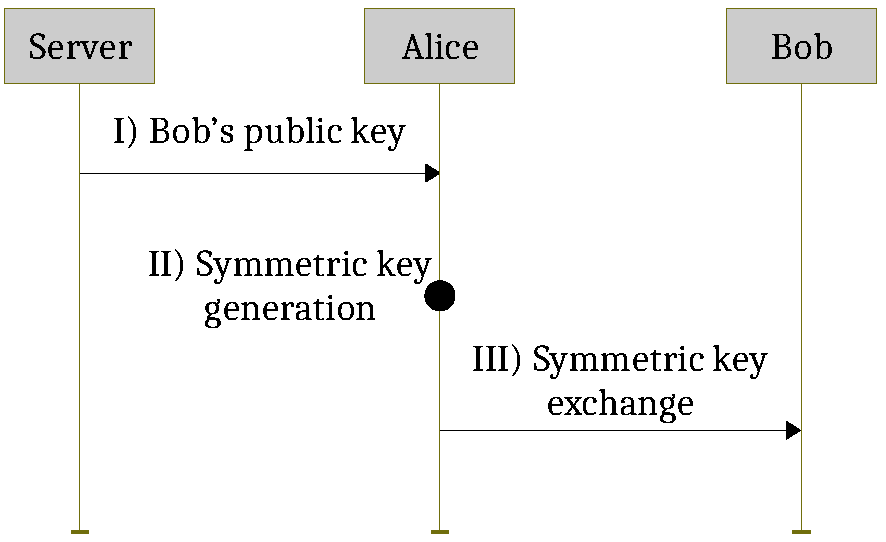
\includegraphics[width=.7\columnwidth]{protocol-example.pdf}
	\caption{Abstraction of an ad-hoc esemplificative protocol execution}
	\label{fig:protocol-example}
\end{figure}
As an illustrative example, in Figure~\ref{fig:protocol-example}, under the perfect
cryptography assumption (i.e. assuming that the cryptographic primitives have
no security flaw), and assuming that no violation to any security property
occurs after message I), the freedom of choosing the scope determines that the
flaws related to the dishonest impersonification of the Server may or may not
be considered in the verification process.  This choice has a tremendous impact
on the focus and findings of the verification of the security of the protocol.
While this may seem to turn upon minutiae and foreseeable, this highlights the
false sense of security that may derive from a non-falsifiable theory of system
security. 
\fix{mr}{In other words, if (as Herley mentions in \autocite{herley}) 
the problem is in the way we reason on cybersecurity, we should
see it in the way we reply to simple cybersecurity (foundamental) questions.
Let us consider the foundamental question ``what is cybersecurity?'',
as in \autocite{hintikka}, we can translate the wh-question into an equivalent
existentially quantified formula. 
But if the formula is the following second-order formula: $\exists P. P(s)\rightarrow Secure(s)$,
(where we ask if there exists a predicate $P$ such that, given any arbitrary 
system $s$, when $P$ holds for $s$ then $s$ can be considered secure),
when the answer is (for example) ``if the system is confidential, the
system is secure'' the formula becomes tautological. In fact, $P$ and $Secure$ can 
be considered as semantically equivalent (security is confidentiality and vice-versa).}
Instead of starting from reasoning on what makes a system secure or insecure,
we reason on what causes insecurities.
\fix{mr}{We focus on insecurities only caused by the exploitation of
cybersecurity attacks, and we assume that achieving security means preventing all those attacks 
from being exploitable or exploited.}
Our hypothesis is that cybersecurity attacks are only caused by 
the presence of errors in the design or implementation of a system.
For example, a design or implementation error in a sanitization function
may allow an attacker to perform SQL-injections. If errors are necessary
to enable cybersecurity attacks, a theory that predicts all potential 
errors (or source of errors) can be effectively used to predict the
security of a system.
\fix{mr}{Therefore, 
a possible answer to the initial question can be that cybersecurity is the 
absence of attacks and the absence of errors implies cybersecurity.
This, however, raises another question: ``which are all the errors
in (the engineering of) a system that make it possible for a cybersecurity attack
to happen?''. More rigorusly, which scientific theory predicts all
possible errors that causes cybersecurity attacks? 
}

With our approach, a list of weaknesses emerges
from the mathematical formulation of the system and predicts 4 main classes
of weaknesses. Those classes of weaknesses are used to calculate
all the insecurity configurations of all the components of a system,
obtaining a precise estimation of all potential cybersecurity-related risks
in any given system. Our hypothesis can be falsified by means of experiments,
testing if all the predicted weaknesses are present in the system under
test, or testing if other (not predicted by our hypothesis) weaknesses are
present.


\paragraph{Structure} 
We start, in Section~\ref{sec:literature}, by detailing the problem statement,
reporting a literature review on the main concepts and definitions related to
security.  We formulate a security hypothesis in Section~\ref{sec:hypothesis};
which we use to propose a theory on system security in
Section~\ref{sec:theory}. In Section~\ref{sec:secra}, we apply our theory for
the tool-assisted security risk assessment of a Cyber-Physical System (CPS), with an ad-hoc example,
based on the SWaT testbed \autocite{Mathur2016swat}.  This application shows
how our theory can be used to predict all of the possible security weaknesses
of a system, allowing the falsification of our theory.  In fact, if any
security weaknesses were to be found in a system and not predicted by our
theory, the theory could be declared incomplete.  Similarly, if a security
weakness would be predicted by our theory but found to be impossible to
realize, our theory could be declared as wrong.

\section{Literature Review}\label{sec:literature}
\begin{figure*}[t]
	\centering
	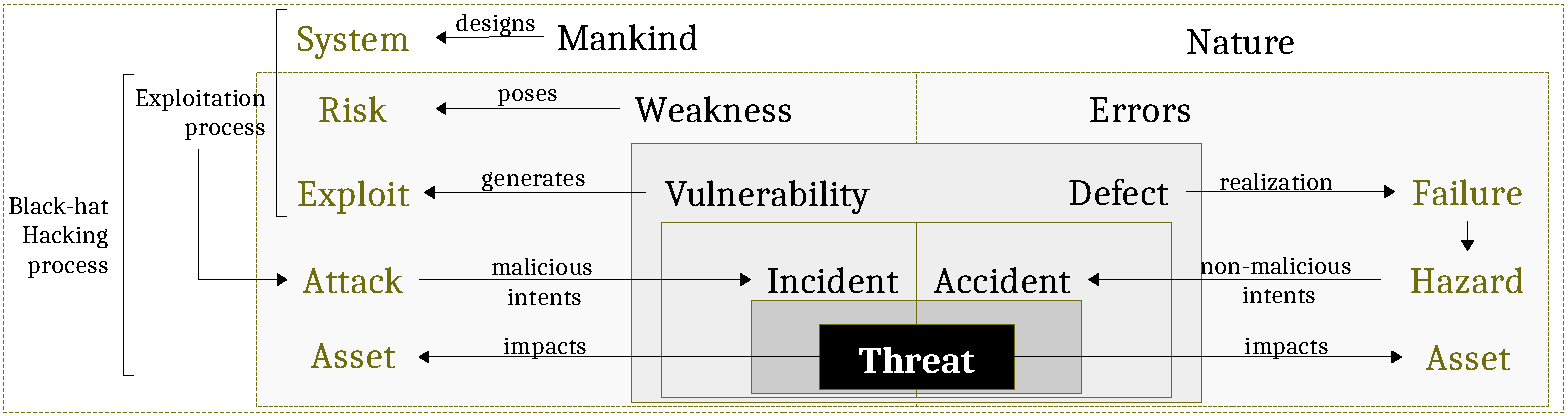
\includegraphics[width=.8\textwidth]{safety-security_3.pdf}
	\caption{Overview of keywords related to security and safety}
	\label{fig:safety-security}
\end{figure*}

In most of the natural languages the concepts of safety
and security are not syntactically differentiated and both terms (safety and
security) are expressed by the same word, e.g. sicurezza in Italian.  A
semantic distinction between safety and security is correlated to a
belief\footnote{A belief has to be intended as a proposition which is supposed
to be true by the majority of people in our society, without a scientific
underlying theory but based on partial empirical evidences or inductive reasoning based on partial empirical evidences.} that
safety deals with \emph{accidents} (i.e. an unfortunate incident) posed by the
natural environment (e.g. natural events such as wearing of hardware
components), whereas security deals with \emph{incidents} posed by mankind (e.g.
attackers and bugs). The fundamental difference between nature and mankind (and,
in turn, between safety and cybersecurity) is believed to be on the different
intents (incidents are intentional, whereas accidents are not) of the causes
that generates a threat. Namely, nature is believed not to have malicious
intents (but unfortunate causes-effects), whereas threats generated by mankind are
malicious\footnote{Of course, logical flaws or bugs may be
introduced by other means (e.g. ignorance) without explicit malicious intents,
but the exploitation of those flaws is considered (for now, and detailed
afterwards in the article) malicious, and thus we consider any vulnerability to
be malicious even if it is due to the lack of skills.}.
This conclusion seems to be against a general formulation of a cybersecurity theory;
how can we define a theory that predicts what a human being will do?
Cybersecurity attacks seem to be related to the creativity of the attacker
and thus unpredictable. 

Currently, the most complete understanding of insecurity issues, is stored into
a network of databases of weaknesses (e.g.
CWE~\autocite{MITRE2020CWEresearch}), vulnerabilities (e.g. CVE~\autocite{CVE},
NVD~\autocite{NIST2020NVD}), and attacks (e.g. CAPEC~\autocite{MITRE2020CAPEC},
ATT\&CK~\autocite{MITRE2020ATTACK}).  Those insecurity issues can be related to
the violation of one or more requirements (explicit or implicit) in the
specification, design or implementation of a system. The correlation 
between insecurity flaws and security requirements has been used to define
standards such as the IEC 62443-1-3 (the Industrial communication networks -
Network and system security -- Part 3-3: System security requirements and
security levels) which defines requirements as ``confidentiality of information
in transit/at-rest''. More generally, the idea of defining security requirements
as properties of a system was initially defined in 1970s with the 
CIA triad (Confidentiality, Integrity, Availability) and refined 
over the decades introducing related concepts such as authenticity or
non-repudiation, or introducing new ones such as ``responsibility'' in the
RITE approach (see~\autocite{Samonas2014cia} for an overview of the evolution of the CIA triad).
The link between security requirements and vulnerabilities is reported 
in the NVD databases by the CVSS\autocite{Mell2007CVSS}) scoring system.
The CVSS evaluates of the severity of a vulnerability
by means of different metrics (such as attack complexity and user interaction)
and quantitatively evaluates the impact on the CIA triad.
While security requirements, weaknesses, vulnerabilities, and attacks
have been extensively studied and implemented both in academia and industry
to provide tools for the testing or verification of systems, 
no scientific falsifiable theory correlate
security requirements to necessary and sufficient conditions (e.g. mitigations) 
to declare a system secure \autocite{Herley2016unfalsifiability}.
Nonetheless, the extensive body of literature have scientific foundations,
for example, providing either providing necessary or sufficient conditions
for cybersecurity.
As a driver for our argumentation, we start by reviewing the key concepts
in the cybersecurity domain.

\subsection{Terminology}
Most of the safety-preserving principles in the field of engineering of
safety-critical cyber-physical systems (such as elevators and aircraft), upon
which safety requirements are defined (e.g. in standards such as the IEC 61508
or 61511\autocite{IEC201761511}), are based on empirical tests and measurements.
While reasoning by induction
%\footnote{``So, whenever they argue ``Every man is an
%animal and Socrates is a man; therefore Socrates is an animal,'' proposing to
%deduce from the universal proposition ``every man is an animal'' the particular
%proposition ``Socrates therefore is an animal,'' which in fact goes (as we have
%mentioned) to establish by way of induction the universal proposition, the
%fall into the error of circular reasoning, since they are establishing the
%universal proposition inductively by means of each of the particulars and
%deducing the particular proposition from the universal syllogistically.''
%Sextus Empiricus, Outlines of Pyrrhonism II-195 \autocite{Empiricus1990Pyrrhonism}}
based on the empirical observation should be avoided in general,
since it may easily lead to false beliefs \autocite{Popper1959logic}, 
inducing general principle by means of tests
is often justified by the supposed impossibility of defining a theory
that correctly predicts failures.
A failure of a wire due to environment (e.g. due to humidity,
dust, heat \&c) is defined from empirical evidences and processes have been
standardized to test qualities of hardware components.  This process completely
breaks down when a malicious environment (i.e. an attacker) is considered
instead of the (supposedly honest and predictable) natural environment.
Therefore, the same approach that is in use for safety, seems not to be
applicable for cybersecurity (e.g. for cybersecurity testing).  An overview on the
aforementioned aspects of safety and cybersecurity is depicted in
Figure~\ref{fig:safety-security} and is used as a baseline for a definition of
the terms that structure our current understanding of cybersecurity.
 
\begin{itemize}
	\item \emph{Mankind} ``refers collectively to humans''
\autocite{wiki-mankind}, while the concept of \emph{Nature} is
		related ``to the intrinsic characteristics that plants,
		animals, and other features of the world develop of their own
		accord'' (e.g. the physical universe)~\autocite{wiki-nature}. 
		\begin{itemize}
			\item There exist several terms to refer to an
				\emph{attacker}, e.g. threat agent or threat source,
				but, from now on, we consider the
				Causality principle to be the \emph{threat
				source}, Nature or Mankind to be the
				\emph{threat agents} and an \emph{attacker} as
				a specific malicious threat agent which materializes a
				threat.
		\end{itemize}
	\item \emph{Vulnerability}\footnote{The term vulnerability is not
		present in the Encyclopedia of Cryptography and Security, while
		it is used in 12 entries (such as in the definition of
		``penetration testing'' \autocite{caddy2005pentest})
		highlighting how commonly this word is used without a proper
		supporting semantics.}, as defined in \autocite{cnssi20104009}
		(and adopted in \autocite{nist2013800-53}), is a ``weakness in an
		information system, system security procedures, internal
		controls, or implementation that could be exploited by a threat
		source''. On the one hand, the definition is broad to enclose
		as much causes (that generates a vulnerability) as possible,
		on the other hand the term vulnerability should have a complete and sound
		definition, so that no other causes (e.g.  other sources) but
		the ones in the definition are responsible for a vulnerability
		%\footnote{``For this view, that
		%\emph{That Which Is Not} exists, can never predominate. You
		%must debar your thought from this way of search, nor let
		%ordinary experience in its variety force you along this way,
		%(namely, that of allowing) the eye, sightless as it is, and the
		%ear, full of sound, and the tongue, to rule; but (you must)
		%judge by means of the Reason (Logos) the much-contested proof
		%which is expounded by me.'' -- Parmenides of Elea, On Nature
		%(circa 500 B.C.), fragments B7.1–8.2
		%\autocite{Hakim2016philosophy}}.
		Furthermore, the term ``threat sources'' used in the definition
		in~\autocite{cnssi20104009} may be identified with both Nature
		and Mankind, not differentiating between safety and security.
\end{itemize}

As depicted in Figure~\ref{fig:safety-security}, a vulnerability does not
necessarily become a threat for the system, unless exploited ``through a
channel that allows the violation of the security policy
[\ldots]''~\autocite{cnssi20104009}. For example, a software or procedure that takes
advantage of the vulnerability causing an \emph{attack} to the system may
result in several correlated incidents and threats.  The process of
exploitation of a defect as a vulnerability is reported in
Figure~\ref{fig:safety-security} such that the difference between exploit and failure,
and attack and accident, is to be found just in the maliciousness of the intents
that causes this process (i.e. excluding the intent, the terms are just syntactic transformation from a vulnerability to defect, from
accident to incident). 

\begin{itemize}
	\item \emph{Weakness}. The definition given by the MITRE in
		\autocite{MITRE2020CWEweakness} of weakness is: `` a type of
		mistake that, in proper conditions, could contribute to the
		introduction of vulnerabilities within that product. This term
		applies to mistakes regardless of whether they occur in
		implementation, design, or other phases of a product
		lifecycle.'' A vulnerability, such as those enumerated on the
		Common vulnerabilities and Exposures (CVE) List, is a mistake
		that can be directly used by a hacker to gain access to a
		system or network.  The definition is circular if we interpret
		the word ``error'' and ``mistake'' with the same semantics: a
		weakness is an error that leads to a vulnerability and a
		vulnerability is a mistake which, in turn, is a weakness. The
		only difference between a weakness and vulnerability seems to
		be that one can consider weakness as a ground term and state
		that a vulnerability is caused by a weakness.
	\item \emph{Causality} refers to the causality principle; defined
		in~\autocite{Spirkin1983Dialectical} as ``Causality is a genetic
		connection of phenomena through which one thing (the cause)
		under certain conditions gives rise to, causes something else
		(the effect). The essence of causality is the generation and
		determination of one phenomenon by another. In this respect,
		causality differs from various other kinds of connection, for
		example, the simple temporal sequence of phenomena, of the
		regularities of accompanying processes''. 
		%One can consider the
		%causality principle to be formalized by the K Modal Logic.
	\item An \emph{Exploit} ``[\ldots]
		(from the English verb to exploit, meaning to use something to
		one’s own advantage) is a piece of software, a chunk of data,
		or a sequence of commands that takes advantage of a bug or
		vulnerability to cause unintended or unanticipated behavior to
		occur on computer software, hardware, or something electronic
		(usually computerized).''~\autocite{wiki-exploit}.
	\item An \emph{Attack}, as defined by the International Standard
		ISO/IEC 27000, is an ``attempt to destroy, expose, alter,
		disable, steal or gain unauthorized access to or make
		unauthorized use of an asset''; where an \emph{Asset} is
		``anything that has value to the organization''. We note that for
		the purpose of this article, we do not want to focus on a specific
		organization or business to define asset but, in general, on any 
		abstract organization (e.g. a company or a society).
		We do not consider ethical hackers as attacking a system. 
		In fact, we consider the term \emph{hack} as
		non-malicious (as, e.g. in~\autocite{Stallman2002hacker}).
	\item A \emph{Threat}, as defined in~\autocite{cnssi20104009}, is ``Any
		circumstance or event with the potential to adversely impact
		organizational operations (including mission, functions, image,
		or reputation), organizational assets, individuals, other
		organizations, or the Nation through an information system via
		unauthorized access, destruction, disclosure, modification of
		information, and/or denial of service''.
	\item \emph{Defect}: ``anything that renders the product not reasonably
		safe''~\autocite{Robinson2019writing} (i.e. a characteristic of
		an object which hinders its proper usability).
	\item \emph{Failure}, as defined in\autocite{Merriam2020failure}, is ``a state of
		inability to perform a normal function''. The term is
		structured and detailed in
		\autocite{cnssi20104009,iet2017glossary}, but relying on an
		abstract notion of failure without a specific definition.
	\item \emph{Hazard}, ``a potential source of
		harm''~\autocite{iet2017glossary}.
\end{itemize}

\begin{figure}[t]
	\centering
	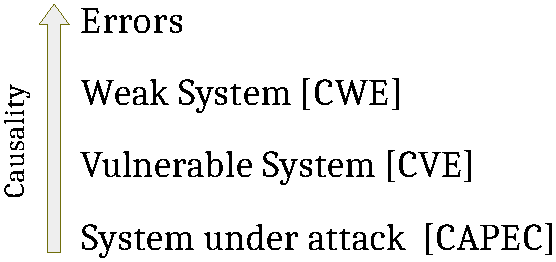
\includegraphics[width=.6\columnwidth]{causality.pdf}
	\caption{Etiology of cybersecurity}
	\label{fig:causality}
\end{figure}

Our literature review shows that most of the definitions relate insecurity to
dis-honesty (also called maliciousness or adversarial) of an agent (often
called adversary or attacker). In fact, weaknesses become vulnerability if an
attacker exploits them in an attack.  This, however, just moves the problem of
defining what cybersecurity is as the problem of defining what a dishonest
agent can or cannot do in a system, where an agent is any virtual or physical
entity of the system or using the system (e.g. a device, a software, or a human
being) and dishonesty is not necessarily related to malicious motivation but
also to incompetence or lack of skills. As in the Dolev-Yao theory, we may
correlate ``being dishonest'' to ``not following the intended behavior/rules''.
In the case of a generic system, a dishonest agent is, therefore, any agent
that doesn't follow the intended behavior (or functionality or logic) of the
system.  For example, a software can be considered an agent of the system and
whenever it has a bug, it can be exploited causing an Incident. However, this
may lead to the conclusion that the dishonest behaviors of agents cannot be
defined in general (e.g. due to the heterogeneity of agents and systems) and
that huge repository of dishonest behaviors should be kept as definition, such
as CAPEC~\autocite{MITRE2020CAPEC}; or that dishonesty of an agent with respect
to a security protocol should be defined as a number of predefined actions as
in
\autocite{Turuani2006clatse,Basin2005ofmc,Armando2016satmc,Rocchetto2017interpolation}
(to name a few)\footnote{In formal protocol verifiers, in the DY model, the
attacker has a set of hardcoded inference rules that defines how the attacker
deduces new messages based on the observed message exchange.}.  As depicted in
Figure~\ref{fig:causality}, in order to define a theory on cybersecurity we may
say that the presence of vulnerabilities is a necessary condition in order to
cause an Attack in the system.  Those vulnerabilities are, in turn, caused by
the presence of weaknsesses in the system.  Weaknesses are errors in the design
or implementation of a system.  Therefore, a theory on cybersecurity should
first predict the errors in a system design.

\section{Security Hypothesis -- ABF Theory of Agents}\label{sec:hypothesis}
In order to address the problem raised by Herley, we shall define how to
distinguish between a secure and an insecure system. While most of the
literature have correlated the problem of in-security
to the maliciousness of agents interacting with the system, we show that
security doesn't seem to stem from a malicious nature but, rather, insecurity
raises from the lack of well-defined security requirements for the development
process of a system. We argue that the high number of security vulnerability
reported today are simply the realization of potential system configurations,
which deviate from the nominal behavior because the \emph{intended (or
nominal) behavior} of the system is not precisely defined in the specification
at the very early stages of the engineering process.

As a reference, we consider the following steps of the engineering process
and our objective is to be able to predict the security requirements
instead of axiomatically assume them.
\begin{enumerate}
	\item \emph{System Specification}, where the \emph{functional and physical requirements} are defined
	\item \emph{Architecture Design}, where the specification is structured into \emph{functional and physical architectures}
	\item \emph{Security Risk Assessment}, where the potential \emph{weaknesses} (errors)
		are identified and, consequently, \emph{security requirements} are
		captured.
	%\item \emph{Design Refinement}, where the physical and functional
	%	architectures are extended with \emph{mitigations} for the
	%	weaknesses. Mitigations at this step details the semantics of
	%	the functional blocks (behaviors), the data flow, and communication logic.
	%\item \emph{Verification of Security Requirements}, where the data flow, behaviors, and communication protocols are verified against the security requirements.
\end{enumerate}
Given that, in our investigation, we changed the focus from the attacker to the
potential designs of a system, we start by defining a general framework for the definition
of a system. On top of this framework we will identify system weaknesses as potential
design errors.

\subsection{Epistemology and Multi-Agent Systems}\label{sec:system}
The ISO/IEC/IEEE 15288:2015 (System Life Cycle Processes) provides a definition
of system as ``A combination of interacting elements organized to achieve one
or more stated purposes.''\autocite{ISO201515288}. If a system is structured
into multiple sub-systems, a sub-system can be defined in the same way as a
system is defined (i.e. as a composition of interacting elements). A hierarchy
of sub-systems can be limited by a ``bottom-subsystem'' often called device (or
element in the aforementioned definition) which is not itself composed by other
elements but is considered atomic.         For the sake of simplicity, we
consider a device as a system with only one element: itself.  We then first define a
system as composed by a single element and then extend the definition to a
``combination of interacting'' elements. Given that we use concepts from the
multi-agent system research field, instead of using the word element we will
use the word agent.

There is no agreement between the research communities (e.g.
Multi-Agent-System, Epistemic Logic) on which are the constituent of an agent.
However, the same ideas revolved around for thousands of years.
Some relevant examples for our objective are the following\footnote{
It is interesting to notice that 
in \autocite{Empiricus1990Pyrrhonism}, the author states: ``The
 logical criterion also may be used in three senses -- of the
 agent, or the instrument, or the ``according to what''; the
 agent, for instance, may be a man, the instrument either sense
 perception or intelligence, and the ``according to what'' the
 application of the impression ``according to'' which the man
 proceeds to judge by means of one of the aforesaid
 instruments.''. The author than proceeds showing that
 even in this framework, knowledge still is non-apprehensible.
}.
\begin{itemize}
	\item In \autocite{Hintikka1962knowledge}, Hintikka describes the
		difference between knowledge and belief (as epistemological
		concepts), and the whole Doxastic logic defines in details how
		beliefs can be formalized.
	\item In \autocite{Hintikka1993Information}, Hintikka describes the concept
		of information and the difference with knowledge and belief.
	\item In \autocite{Santaca2016abf}, the authors defines an agent as a
		tuple of assertions, beliefs, and facts.
\end{itemize}
For our argument, as in \autocite{Santaca2016abf}, an agent is composed by its
knowledge, beliefs, and the information or assertions it provides; where
knowledge is defined, as in \autocite{Steup2020epistemology}, as a set of
proposition known by an agent, such that: (i) knowledge requires belief, (ii)
knowledge require truth, (iii) knowledge must be \emph{properly justified}, and
the only objective of information is to exchange beliefs between agents.  As
defined in \autocite{Hintikka1993Information}, ``information is specified by
specifying which alternatives concerning the reality it admits and which
alternatives excludes''. This means that if we consider a propositional
variable (which admits the two alternatives True/False) its information is
defined as Believed to be True/False and not Believed to be the opposite.  Due
to the definition of information and then with its relation to the
probabilistic correlation to truth/reality, we consider information in relation
with an agent's beliefs. Similarly, we consider beliefs to define the actual
behavior of an agent or a system; i.e. we consider behaviors as belief revision
systems.
The difference between knowledge and information as used by Hintikka, and facts
and assertions as used in \autocite{Santaca2016abf}, are not precisely discussed
in \autocite{Santaca2016abf}.  Furthermore, those epistemological concepts are
difficult to define
\autocite{Gettier2012knowledge}.
%\footnote{``\emph{Theaetetus}: [\ldots] He said
%that knowledge was true opinion accompanied by reason, but that unreasoning
%true opinion was outside of the sphere of knowledge; and matters of which there
%is not a rational explanation are unknowable -- yes, that is what he called
%them -- and those of which there is are knowable. [\ldots] \emph{Socrates}:
%[\ldots] the primary elements of which we and all else are composed admit of no
%rational explanation; for each alone by itself can only be named, and no
%qualification can be added, neither that it is nor that it is not, for that
%would at once be adding to it existence or non-existence, whereas we must add
%nothing to it, if we are to speak of that itself alone.  [\ldots]'' Plato --
%Theaetetus 201 \autocite{Plato1914Plato}}.
For example, Hintikka in
\autocite{Hintikka1993Information} states that ``A purely logical definition of
information is impossible''. However, a detailed formalization of those concepts is out
of the scope of this paper. 

We now define those concepts abstractly, inspired by the
$\abftheory$-framework  defined in \autocite{Santaca2016abf} and, in
Section~\ref{sec:theory} we detail them as engineering concepts.
\begin{enumerate}
	\item We consider information only when the intention of exchanging 
		that information is from a sender to 
		recipient is defined; and we call it \emph{assertion}  
	\item Similarly, the portion of \emph{beliefs} we consider for system
		engineering is the one that builds (input) or describes
		(output) the behavior of an agent (strategy rules
		\footnote{``The logical structure of information is one of the
		most basic and one of the most basic and one of the simplest
		thing in the wide and wonderful world of logical analysis. This
		point can be put in a deeper perspective. A distinction
		[\ldots] ought to be made [--] between two kinds of rules (or
		principles) in any strategic activity like knowledge seeking.
		On the one hand you have the rules that define the game, e.g.
		how chessmen are moved on a board. The can be called
		\emph{definitory} rules.  They must be distinguished from rules
		[\ldots] that deal with what is better and what is worse in the
		game in question.  Definitory rules do not say anything about
		this subject. Rules which do can be called \emph{strategic
		rules}'' -- Hintikka in \autocite{Hintikka1993Information}}),
		and
	\item We consider a set of axiomatic \emph{facts} (definitory
		rules\footnote{Facts are definitory rule as they don't
		define how a real system is finally implemented but
		how it should be, trough a series of requirements. Those requirements 
		may not hold, through insecurity, in the implemented system.})
		instead of considering the more general epistemic definition of
		knowledge. Specifically, facts describes:
		\begin{itemize}
			\item The functional architecture of each agent
			\item The physical/structural (HW/SW) architecture of each
				subsystem of agents and agent within a
				subsystem
		\end{itemize}
\end{enumerate}
We give a graphical representation of (sub-)system and agent in Figure~\ref{fig:system-agent}.
The notation will be introduced in the next section but, intuitively,
Figure~\ref{fig:system-agent} shows a system composed by two agents. The system
has two ports denoted by ``I'' (with incoming assertions) and ``O'' (with outgoing assertions).
The bottom part of Figure~\ref{fig:system-agent} details the structure of a single
agent which is not decomposed into other (sub-)agents. In this case, ports translates
incoming assertions into beliefs that feeds the behavior block, and outgoing beliefs
from the behavior block are then translated back into (outgoing) assertions.

\begin{figure}[t]
	\centering
	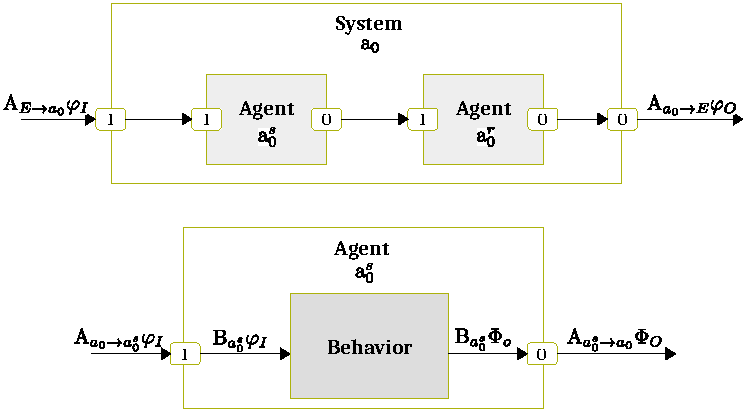
\includegraphics[width=.9\columnwidth]{system-agent.pdf}
	\caption{Example of system and agent structure}
	\label{fig:system-agent}
\end{figure}

\subsection{Mereo-topological Reasoning}
\begin{table*}[t]
\centering
\begin{tabular}{ccclll} 
\rota{\textbf{RCC3}}&\rota{\textbf{RCC5}}&\rota{\textbf{RCC8}}&\textbf{Terminology} & \textbf{Notation} & \textbf{Definition} \\
\hline
&&&Connects with 			& $\mathit{C}(\mathit{X},\mathit{Y})$ 		& $\mathit{X}\subseteq \mathit{Y}$ \\
&&&Disconnected from		& $\neg \mathit{C}(\mathit{X},\mathit{Y})$		& $\mathit{X}\not\subseteq \mathit{Y}$\\
&&&Part of				& $\mathit{P}(\mathit{X},\mathit{Y})$		& $\forall \mathit{Z} ~\mathit{C}(\mathit{Z},\mathit{X}) \rightarrow \mathit{C}(\mathit{Z},\mathit{Y})$\\
&&&Overlaps			& $\mathit{O}(\mathit{X},\mathit{Y})$		& $\exists \mathit{Z} ~\mathit{P}(\mathit{Z},\mathit{X})\wedge \mathit{P}(\mathit{Z},\mathit{Y})$\\
\Tdot&&&  \textbf{Overlaps Not Equal} 	& $\mathit{ONE}(\mathit{X},\mathit{Y})$		& $\mathit{O}(\mathit{X},\mathit{Y}) \land \neg \mathit{EQ}(\mathit{X},\mathit{Y})$ \\
\Tdot&\Tdot&\Tdot& \textbf{Equal to} 		& $\mathit{EQ}(\mathit{X},\mathit{Y})$  		& $\mathit{P}(\mathit{X},\mathit{Y}) \wedge \mathit{P}(\mathit{Y},\mathit{X})$\\
\Tdot&\Tdot&\Tdot& \textbf{DiscRete from} 		& $\mathit{DR}(\mathit{X},\mathit{Y})$		& $\neg \mathit{O}(\mathit{X},\mathit{Y})$\\
&\Tdot&\Tdot&\textbf{Partial-Overlap}	& $\mathit{PO}(\mathit{X},\mathit{Y})$ 		& $\mathit{O}(\mathit{X},\mathit{Y})\wedge \neg \mathit{P}(\mathit{X},\mathit{Y}) \wedge \neg \mathit{P}(\mathit{Y},\mathit{X})$\\ 
&\Tdot&&\textbf{Proper-Part-of} 	& $\mathit{PP}(\mathit{X},\mathit{Y})$ 		& $\mathit{P}(\mathit{X},\mathit{Y})\wedge \neg \mathit{P}(\mathit{Y},\mathit{X})$\\ 
	&\Tdot&&\textbf{Proper-Part-of-\textit{\textbf{i}}nverse} & $\mathit{PPi}(\mathit{X},\mathit{Y})$ 		& $\mathit{P}(\mathit{Y},\mathit{X}) \wedge \neg \mathit{P}(\mathit{X},\mathit{Y})$\\
&&\Tdot&\textbf{Externally Connected} 	& $\mathit{EC}(\mathit{X},\mathit{Y})$ 		& $\mathit{C}(\mathit{X},\mathit{Y}) \wedge \neg\mathit{O}(\mathit{X},\mathit{Y})$\\ 
&&\Tdot&\textbf{Tangential PP} 	& $\mathit{TPP}(\mathit{X},\mathit{Y})$ 		& $\mathit{PP}(\mathit{X},\mathit{Y})\wedge\exists\mathit{Z}~[\mathit{EC}(\mathit{Z},\mathit{X}),\mathit{EC}(\mathit{Z},\mathit{Y})]$\\ 
&&\Tdot&\textbf{Tangential PPi} 	& $\mathit{TPPi}(\mathit{X},\mathit{Y})$ 		& $\mathit{TPP}(\mathit{Y},\mathit{X})$\\ 
&&\Tdot&\textbf{Non-Tangential PP} 	& $\mathit{NTPP}(\mathit{X},\mathit{Y})$ 		& $\mathit{PP}(\mathit{X},\mathit{Y})\wedge\neg\exists\mathit{Z}~[\mathit{EC}(\mathit{Z},\mathit{X}),\mathit{EC}(\mathit{Z},\mathit{Y})]$\\ 
&&\Tdot&\textbf{Non-Tangential PPi} 	& $\mathit{NTPPi}(\mathit{X},\mathit{Y})$ 		& $\mathit{NTPP}(\mathit{Y},\mathit{X})$\\ 
\end{tabular}
\caption{RCC3, RCC5, and RCC8 relations between regions $X$, $Y$ and $Z$ ~\label{tab:rcc358}~\label{tab:rcc}}
\end{table*}

Similarly to \autocite{Santaca2016abf}, we define agents as a meronomy (an
hierarchy of Part-Whole relations) over the constituent that we previously defined
(assertions, beliefs, and facts), based on a standard definition of mereology,
i.e. based on the definition of parthood relation between \emph{Parts}.  Due to
the necessity of considering different relations between parts (as we'll show afterwards)
we extend the mereology to a
mereo-topology \autocite{Smith1996mereotopology,Varzi1994mereotopology,Rachavelpula2017mereotopology},
considering the relations in Table~\ref{tab:rcc358}.  For the sake of
readability, we use the term \emph{region} both to refer to a mereological Part
and to a topological region.  Our aim is to create a meronomy (hierarchy of part-whole
relations)
instead of the taxonomies (categorization based on discrete sets) 
such as the one provided
in \autocite{NIST2020NVD,MITRE2020CVE} 
so that we don't need to rely on a scoring system (such as the 
CVSS) to assign a quantitative evaluation 
of the security of each entry. Instead, we want a precise calculation
of the number of insecurity configurations to emerge from the mathematical
formulation of our cybersecurity theory.

A mereotopology, as defined e.g. in \autocite{Rachavelpula2017mereotopology},
is an ordered mathematical structure where the basic relation between regions
is the reflexive and symmetric relation \emph{Connects With} $\subseteq$,
that we use to order a universe of agents
$\agentuniverse$ (see in Table~\ref{tab:rcc358}).  We use the Region Connection
Calculus (RCC), as defined in~\autocite{bennettLogics,improvingRCC}, to provide
an axiomatization of the mereo-topological concepts. In its broader definition,
the RCC theory is composed by eight axioms, and is known as RCC8. In the text,
for brevity, we will often focus only on RCC5 without loss of generality. Using
RCC5 instead of RCC8 prevents us from considering tangential connections
between spatial regions. However, tangential connections in RCC8 can be
considered as special cases of the more general spatial relations considered in
RCC5.

In Table~\ref{tab:rcc}, we summarize the axioms of the RCC (see, e.g., \autocite{Grutter2008rcc}).  We can now define a system
over the mereotopology using the RCC calculus, as follows, where $\rcc(X,Y)$ on
two generic regions $X,Y$ represents one of the possible RCC relations between
$X$ and $Y$. We note that all the RCC relations are symmetric with the exception
of those that has an explicit (related) inverse.

\begin{definition}{\bf System State --}\label{def:opsystem}
	A CPS system (or a sub-system) state is defined as the tuple
	$s=\langle\rcc(\factRegion,\beliefRegion),\rcc(\factRegion,\assertionRegion),\rcc(\beliefRegion,\assertionRegion)\rangle$,
	where $\assertionRegion,\beliefRegion,\factRegion$, are regions of
	assertions, beliefs (i.e. the beliefs generated by the behavior), and
	facts expressed as requirements respectively.
\end{definition}

As already presented in \autocite{Santaca2016abf} it follows that, defining
a system with a fixed number of regions, there exist
an upper-bound to the number of possible configuration of a system, defined by
the possible relations between the different regions.
For completeness, we report in the next paragraph 
the calculation done in \autocite{Santaca2016abf}.

\paragraph{Number of different configurations of a system}
The general formula to calculate the number of different types of agents is
$r^{\binom{n}{k}}$, where $r$ is the number of relations with arity $k$,
between $n$ different regions. Therefore, $r^{\binom{n}{k}}$
expresses the number of permutation of $r$
relations over ${\binom{n}{k}}$ elements with repetitions, 
with ${\binom{n}{k}}$ being the number of
$k$-ary combinations of $n$ regions.
In our case, $\binom{n}{k}=3$ since we consider $3$ regions 
($\assertionRegion,\beliefRegion,\factRegion$), and all the relations
considered in the RCC are binary.  Hence, using RCC5 (with five different
spatial relations) over three regions, we can theoretically define up to 125
different type of agents. However, only 54 of the 125 (as showed in
\autocite{improvingRCC}) combinations are topologically correct with respect to
the definition of the relations of RCC5. Generalizing to all the RCCs:

\begin{itemize}%[nosep]
\item \emph{RCC3} --- theoretical: $3^3=27$,  correct: 15 
\item \emph{RCC5} --- theoretical: $5^3=125$, correct: 54
\item \emph{RCC8} --- theoretical: $8^3=512$, correct: 193
\end{itemize}

Hence, even if considering a different number of regions than the three
$\assertionRegion$, $\beliefRegion$, and $\factRegion$ exponentially affects
the number of theoretical agents, the application of RCC downscales that number
of a factor that ranges from 1.8 to 2.5. In addition, using RCC5 we consider
3.6 times more (different) types of agents than RCC3, but using RCC8 would
allow us to consider 3.5 times more different agents.
In the quantitative evaluation of a single agent, depicted in Figure~\ref{fig:quantitative},
we argue that only 1 configuration represents the nominal (expected) behavior 
of the agent while the other configurations are either impossible to 
implement or diverge from the intended nominal behavior. We note 
that, the numbers reported here do not consider the details of the
engineering process and should be considered a limit of an abstract 
representation of the system.
\begin{figure}[t]
	\centering
	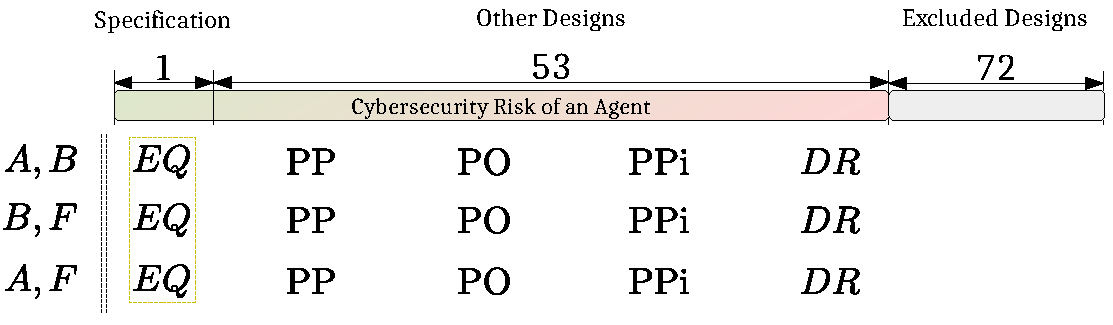
\includegraphics[width=\columnwidth]{quantitative.pdf}
	\caption{Cybersecurity risk for a single agent}
	\label{fig:quantitative}
\end{figure}

\subsection{Qualitative Evaluation of Agent Space in $\abf$}\label{sec:agentspace}
\begin{table}[t]
\centering
\begin{adjustbox}{width=\columnwidth}
\begin{tabular}{r||c|c|c|c|c} 
& \dr{$\assertionRegion$}{$\beliefRegion$} & 
	\po{$\assertionRegion$}{$\beliefRegion$}& 
	\pp{$\assertionRegion$}{$\beliefRegion$} &
	\ppi{$\assertionRegion$}{$\beliefRegion$} & 
	\eq{$\assertionRegion$}{$\beliefRegion$} \\
\hline
\hline %dr
 \multirow{3}{*}{\dr{$\beliefRegion$}{$\factRegion$}} & 
	\cellcolor{abfred} & %dr
	\cellcolor{abf-rg-1}\dr{$\assertionRegion$}{$\factRegion$} & %po
	\cellcolor{abf-rg-2}\multirow{3}{*}{\dr{$\assertionRegion$}{$\factRegion$}} & %pp
	\cellcolor{abf-rg-3} \dr{$\assertionRegion$}{$\factRegion$}& % ppi
	 \cellcolor{abf-rg-4} \\ % eq
& \cellcolor{abfred}\all{$\assertionRegion$}{$\factRegion$}& %dr
	\cellcolor{abf-rg-1}\po{$\assertionRegion$}{$\factRegion$} & %po
	\cellcolor{abf-rg-2}\dr{$\assertionRegion$}{$\factRegion$} & %pp
	\cellcolor{abf-rg-3}\po{$\assertionRegion$}{$\factRegion$} & %ppi
	\cellcolor{abf-rg-4}\dr{$\assertionRegion$}{$\factRegion$}\\ % e q
% & \cellcolor{abfred}& %dr
%	\cellcolor{abf-rg-1}& %\pp{$\assertionRegion$}{$\factRegion$} & %po
%	\cellcolor{abf-rg-2}  & %pp
%	\cellcolor{abf-rg-3} & %\pp{$\assertionRegion$}{$\factRegion$} & %ppi
%	\cellcolor{abf-rg-4} \\ %eq
\hline %po
 \multirow{3}{*}{\po{$\beliefRegion$}{$\factRegion$}} &
	\cellcolor{abf-rg-1}\dr{$\assertionRegion$}{$\factRegion$} & %dr
	\cellcolor{abf-rg-2} & %po
	\cellcolor{abf-rg-3}\dr{$\assertionRegion$}{$\factRegion$} & %pp
	\cellcolor{abf-rg-4}\po{$\assertionRegion$}{$\factRegion$} & %ppi
	\cellcolor{abf-rg-5} \\ %eq
 & \cellcolor{abf-rg-1}\po{$\assertionRegion$}{$\factRegion$} & %dr
	\cellcolor{abf-rg-2} \all{$\assertionRegion$}{$\factRegion$} & %po 
	\cellcolor{abf-rg-3}\po{$\assertionRegion$}{$\factRegion$} & %pp
	\cellcolor{abf-rg-4}\ppi{$\assertionRegion$}{$\factRegion$} & %ppi
	\cellcolor{abf-rg-5} \po{$\assertionRegion$}{$\factRegion$}\\%eq
 & \cellcolor{abf-rg-1}\pp{$\assertionRegion$}{$\factRegion$} & %dr
	\cellcolor{abf-rg-2} &  %po
	\cellcolor{abf-rg-3}\pp{$\assertionRegion$}{$\factRegion$} & %pp
	\cellcolor{abf-rg-4}& %ppi
	\cellcolor{abf-rg-5}\\ %eq
\hline %pp
 \multirow{4}{*}{\pp{$\beliefRegion$}{$\factRegion$}} &
	\cellcolor{abf-rg-2}\dr{$\assertionRegion$}{$\factRegion$} & 
	\cellcolor{abf-rg-3}&
	\cellcolor{abf-rg-4} & %pp
	\cellcolor{abf-rg-5}\po{$\assertionRegion$}{$\factRegion$} & %ppi
	\cellcolor{abf-rg-6}\\ %eq
 & \cellcolor{abf-rg-2}\po{$\assertionRegion$}{$\factRegion$} & 
	\cellcolor{abf-rg-3}\po{$\assertionRegion$}{$\factRegion$} & 
	\cellcolor{abf-rg-4}\pp{$\assertionRegion$}{$\factRegion$} & %pp
	\cellcolor{abf-rg-5}\eq{$\assertionRegion$}{$\factRegion$} & %ppi
	\cellcolor{abf-rg-6}\pp{$\assertionRegion$}{$\factRegion$} \\ %eq
 & \cellcolor{abf-rg-2}\pp{$\assertionRegion$}{$\factRegion$} & 
	\cellcolor{abf-rg-3}\pp{$\assertionRegion$}{$\factRegion$} & 
	\cellcolor{abf-rg-4} & %pp
	\cellcolor{abf-rg-5}\pp{$\assertionRegion$}{$\factRegion$} & %ppi
	\cellcolor{abf-rg-6} \\ %eq
 & \cellcolor{abf-rg-2}&
 	\cellcolor{abf-rg-3} & 
	\cellcolor{abf-rg-4}& %pp
	\cellcolor{abf-rg-5}\ppi{$\assertionRegion$}{$\factRegion$} & %ppi
	\cellcolor{abf-rg-6} \\ %eq
\hline %ppi
 \multirow{3}{*}{\ppi{$\beliefRegion$}{$\factRegion$}} &
 	\cellcolor{abf-rg-3}\multirow{3}{*}{} &
 	\cellcolor{abf-rg-4}\dr{$\assertionRegion$}{$\factRegion$} &
 	\cellcolor{abf-rg-5}& %pp
 	\cellcolor{abf-rg-6}& %ppi
 	\cellcolor{abf-rg-7} \\ %eq
& \cellcolor{abf-rg-3}\dr{$\assertionRegion$}{$\factRegion$} &
 	\cellcolor{abf-rg-4}\po{$\assertionRegion$}{$\factRegion$} & 
 	\cellcolor{abf-rg-5}\all{$\assertionRegion$}{$\factRegion$}& %pp
 	\cellcolor{abf-rg-6}\ppi{$\assertionRegion$}{$\factRegion$}& %ppi
 	\cellcolor{abf-rg-7}\ppi{$\assertionRegion$}{$\factRegion$}\\ %eq
& \cellcolor{abf-rg-3} & 
	\cellcolor{abf-rg-4}\ppi{$\assertionRegion$}{$\factRegion$} & 
	\cellcolor{abf-rg-5} & %pp
	\cellcolor{abf-rg-6}& %ppi
	\cellcolor{abf-rg-7}\\ %eq
\hline %eq
	\eq{$\beliefRegion$}{$\factRegion$} & 
	\cellcolor{abf-rg-4}\dr{$\assertionRegion$}{$\factRegion$} & 
	\cellcolor{abf-rg-5} \po{$\assertionRegion$}{$\factRegion$} & 
	\cellcolor{abf-rg-6}\pp{$\assertionRegion$}{$\factRegion$} & %pp
	\cellcolor{abf-rg-7} \ppi{$\assertionRegion$}{$\factRegion$} & %ppi 
	\cellcolor{abfgreen} \eq{$\assertionRegion$}{$\factRegion$}  %eq
\end{tabular}
\end{adjustbox}
\caption{RCC5 composition table over 3 regions. The results show that there
exist 54 possible relations and the coloring anticipates the ideal risk matrix
(green the secure state with low risk, red the high risk state, and a gradient
of medium risk states). 
\all{$\assertionRegion$}{$\factRegion$} = \{\dr{$\assertionRegion$}{$\factRegion$}, \po{$\assertionRegion$}{$\factRegion$}, \pp{$\assertionRegion$}{$\factRegion$}, \ppi{$\assertionRegion$}{$\factRegion$}, \eq{$\assertionRegion$}{$\factRegion$}\}
\label{tab:5com}}
\end{table}
While a quantitative analysis reveals how many possible configurations of an
agent (i.e. a system) exist w.r.t. the $\abf$ theory (i.e. $54/125$ in RCC5), a
qualitative analysis of the different configurations describe the
configurations allowed by the $\abf$ theory, and how those configurations can
be categorized.  In Table~\ref{tab:5com}, we provide the generic composition
table of RCC5 over 3 regions instantiated over $\abf$, which shows the whole
state space for a single agent. The color coding of the table represents the
security risk related to a generic agent, the risk is highest on the top left
corner of the matrix, lowest on the bottom right corner. 

In Figure~\ref{fig:soundness}, the relation between facts, and assertions and
beliefs (as inputs and outputs of the behavior of an agent) is illustrated.
Assertions and beliefs generated by the design of a system may not be exactly
aligned with what the facts mandate (i.e. what the specification mandates).
The relation between facts, and assertions and beliefs can be used as a metric
to determine the soundness of the design with respect to the specification.

We categorize agents by first analyzing the relations between each pair of
regions defining an agent (i.e.  $\abf$), and then we categorize the different
agents as tuple of the three regions.  For the sake of simplicity, soundness is
opposed to non-soundness in the following, however, with the RCC one should
consider different ``degrees'' of non-soundness.  For example, in RCC5, if we
consider EQ between two regions as representing soundness, DR over the same
regions represents non-soundness; while PP, PO, PPi represents the different
degrees of non-soundness.  A similar argument can be done for completeness.  
\begin{figure}[t]
	\centering
	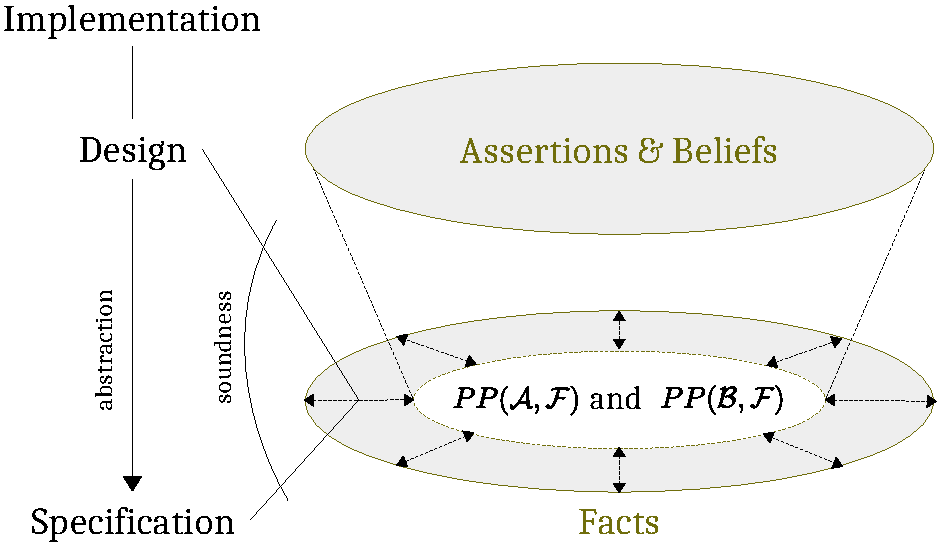
\includegraphics[width=.9\columnwidth]{soundness.pdf}
	\caption{Example relation between facts, and assertions and beliefs}
	\label{fig:soundness}
\end{figure}

\paragraph{\Rcc{$\assertionRegion$}{$\beliefRegion$} -- Collaboration} In order
to reason on the relation between assertions and beliefs we first need to
consider that, by definition, assertions are defined as transfer of information
between two agents, e.g., $a$ and $b$.  Therefore, as depicted in
Figure~\ref{fig:system-agent}, an agent has two main categories of assertions,
input and output assertions.  Given an agent $a$ and a collection of asserted
predicates $\Phi$, the Input assertions are those received by $a$ from an agent
$s$ acting as a sender, $\rassert{s}{a}{\Phi}$; similarly, output assertions
are sent from $a$ to a receiver $r$, $\rassert{a}{r}{\Phi}$. We shall consider
two pairs of regions\footnote{``I am not asserting, as Lotze did, that a
relation between $X$ and $Y$ consists of a quality in $X$ and a quality in $Y$
-- a view which I regard as quite indefensible. -- I assert that a relation $Z$
between $X$ and $Y$ involves the existence in $X$ of the quality ``having the
relation $Z$ to $Y$'' so that a difference of relations always involves a
difference in quality, and a change of relations always involves a change of
quality.'' --  Ellis J. McTaggart, The Unreality of
Time\autocite{Mctaggart1908unreality}}: 
\begin{itemize}
	\item \Rcc{$\assertionRegion_{s\rightarrow a}$}{$\beliefRegion$},
		where the relation between Input-assertions and beliefs
		describes the soundness of the execution of the functional
		architecture w.r.t. input elicitation. With more details, the
		ideal specification of the functional architecture, along with
		the expected inputs, defines the functional behavior of an
		ideal system.  If all the inputs (assertions) are correctly
		handled in the functional specification (beliefs) the
		specification is complete. 

	\item \Rcc{$\assertionRegion_{a\rightarrow r}$}{$\beliefRegion$},
		where the relation between behavior and outputs describes the
		completeness of the behavior defined in the specification
		w.r.t. the input elicitation.  With more details, if all the
		outputs (assertions) of the functional architecture can be
		produced, the functional architecture is complete.
\end{itemize}


\paragraph{\Rcc{$\assertionRegion$}{$\factRegion$} and
\Rcc{$\beliefRegion$}{$\factRegion$} -- Honesty and Competence} 
The relation of assertions
and beliefs with facts determines the quality with respect to the nominal
(specified) system.  Given that facts defines what needs to be true in the system,
the relation of assertions an facts determines the degree of quality between
the real information circulating in a system (or within an agent) and
the one specified.  Since the transfer of information
through assertions generates beliefs, a dishonest agent may circulate false
information, generating false beliefs.  We note that it is often implied that
the intention behind circulating false information discerns a dishonest and an
incompetent agent. However, we consider honesty related to sharing
truths\footnote{``[\ldots] truth exists only in the good man, but the true in
the bad man as well; for it is possible for the bad man to utter something
true.'' Sextus Empiricus, Outlines of Pyrrhonism,
II-83\autocite{Empiricus1990Pyrrhonism}}.  The relation between beliefs and
facts determines the competence (on the subjects defined by the facts) of an
agent (i.e. the more competent an agent is, the more likely a belief of that
agent is true).

\subsubsection{$\abf$ Security Enumeration (SE)} The following security
requirement for a CPS specification can be summarized:
\begin{enumerate}
	\item[SE-$1$] Proper interaction between correctly-behaving agents is
		defined as $\eq{\assertionRegion_a}{\beliefRegion_a}$ for an
		agent $a$ while can be detailed as follows when multiple agents
		are considered.
	\begin{enumerate}
		\item[SE-$1.1$] The equality relation
			$\eq{\assertionRegion_{s\rightarrow
			a}}{\beliefRegion_a}$ describes the intended secure
			behavior as: the beliefs generated by the behavior of
			the functional architecture shall be complete w.r.t.
			the specified inputs of the agent. Therefore, \emph{the
			assertions received by an agent or a system shall be
			compliant with the expected inputs of the functional
			architecture}. For example, the inputs of the user of a
			SW must be sanitized to exclude deviations w.r.t. the
			expected inputs of the functions implemented in the SW.
			Another example is the type checking between allowed
			inputs and expected inputs.
		\item[SE-$1.2$] Similarly, the equality relation
			$\eq{\assertionRegion_{a\rightarrow
			r}}{\beliefRegion_a}$ defines that the outputs of an
			agent $a$ shall be the outputs of the functional
			architecture.
	\end{enumerate}
\item[SE-$2$] The proper adherence of the data transmitted between agents with respect to
	requirements, is defined as $\eq{\assertionRegion}{\factRegion}$. 
\item[SE-$3$] The proper adherence of the behavior (in terms of input and output beliefs) with respect to
		requirements is defined as $\eq{\beliefRegion}{\factRegion}$.
\end{enumerate}

We note that our SE define the properties of a secure system, and correlated
weaknesses can be found in the CWE dataset.  For example, SE-$1$ can be sees as
correlated to the weakness class of ``Improper Interaction Between Multiple
Correctly-Behaving Entities'' defined by the CWE--$435$, SE-$2$ with the
``Insufficient Control Flow Management'' defined by MITRE in the CWE--$691$,
and SE-$3$ with the ``Improper Calculation'' defined by MITRE in the
CWE--$682$. All those CWE are in the top ``view'' of the ``research concepts''
in\autocite{MITRE2020CWEresearch}, while the other classes of weaknesses do not
have a direct counterpart in our theory; we believe they can be sees as sub-classes,
but a full comparison with the CWE is out of the scope of this article.

We are now in the position to define what a secure system is (with respect to
the $\abftheory$-framework) and, based on that definition, what the security risk is and
how to quantify it in a risk matrix.
\begin{definition}{\bf Security of a System or an Agent --}\label{def:security}
	A secure system is a system where SE-$1$, SE-$2$, and SE-$3$ holds for
	each agent composing the system.
\end{definition}
The ISO 31000 consider risk as the ``effect of uncertainty on objectives'' and
refers both to positive and negative consequences of uncertainty.
Accordingly, we consider risk as follows. 
\begin{definition}{\bf Risk --}
A risk is the whole space of potential designs of a specification with respect to the
	$\abftheory$-framework.
\end{definition}
The definition of Risk leads to the risk matrix in
Figure~\ref{fig:quantitative}, defined as follows.
\begin{definition}{\bf Risk Matrix --}
	The risk matrix, as summarized in Table~\ref{tab:5com}, is a function of the three relations
	$s=\langle\rcc(\factRegion,\beliefRegion),\rcc(\factRegion,\assertionRegion),\rcc(\beliefRegion,\assertionRegion)\rangle$,
	where the maximum risk is defined by the $DR$ relation between the
	three groups of regions, and the minimum risk by the $EQ$ relation over
	the same regions. In between the two extremes, the granularity of
	possible intermediate configuration is defined by the calculus used
	(RCC5 in our case).
\end{definition}
While a risk matrix is often defined as a function of the 
likelihood and impact of attacks (based on quantitative ad-hoc estimation
of how likely it is that an attacker will exploit one or more vulnerabilities
and what is the magnitude of the incidents produced by this exploitation), we suggest
that security weaknesses are all equally likely to be exploited
if there's a connection between the weakness and the asset that
an attacker wants to impact. Therefore, a risk matrix should
capture the number of insecure configurations of a system, rather
than predicating over likelihoods of weaknesses exploitation.

\section{Prediction of Security Weaknesses}\label{sec:theory}
Several standards mandate a secure-by-design approach in which cybersecurity
shall be considered at the very early stages of the design process.  For
example,
\begin{enumerate}[noitemsep]
	\item DO-326A -- ``Airworthiness Security Process Specification''
		requires a cybersecurity risk assessment of the design and
		``are the only Acceptable Means of Compliance (AMC) by FAA
		\& EASA for aviation cyber-security airworthiness certification,
		as of 2019'' as pointed out by SAE in \autocite{SAE2019DO326A}.
	\item NIST 800-82 \autocite{Stouffer2011guide} -- ``guide to Industrial
		Control System (ICS) Security''
	\item J3061:2016-1 \autocite{SAE2016J3061} -- ``Cybersecurity Guidebook
		for Cyber-Physical Vehicle Systems'' defines ``set of
		high-level guiding principles for Cybersecurity as it relates
		to cyber-physical vehicle systems'' and states that
		``incorporate Cybersecurity into cyber-physical vehicle systems
		from concept phase through production, operation, service, and
		decommissioning''
\end{enumerate}
However, standards do not describe in detail how to perform a security risk 
assessment and only vaguely define the overall objective, which
can be summarized as to provide an understanding of the potential security risks.
Roughly speaking, a security risk assessment (e.g. CORAS \autocite{Lund2010model}) 
methodology starts from the (i) identification of assets, (ii) determines
the threat scenarios (correlating vulnerabilities, threats and incidents) e.g. 
threat diagrams in the CORAS
approach, (iii) calculates the risk as a function
of impact and likelihood of threat scenarios, and (iv) finally provides
treatments (mandating a partial re-design) and residual risks.
All the methodologies and tools we reviewed (e.g. Threatmodeler \autocite{Threatmodeler},
CORAS \autocite{Lund2010model}, SECRAM \autocite{De2015role})
rely on the expertise of the person who performs the risk assessment for
the identification of threats and for the quantitative estimation of risks.
As Herley puts it \autocite{Herley2016usenixvideo}, ``we don't have a test for security and
we don't have a metric for security'' while standards require a security risk assessment
which, in turn, mandates a metric to evaluate the security risk. 
In contrast, in this section, we define how to specify a CPS in the $\abftheory$-framework
and we identify a security metric.

So far, we have reasoned on systems in the abstract, considering
generic Multi-Agent System (MAS); mapping Epistemological concepts
to MAS. We now map MAS to CPS and show how this mapping allows us
to predict security weaknesses in a system.

\subsection{From Multi-Agent to Cyber-Physical Systems}
\begin{figure*}[t]
	\centering
	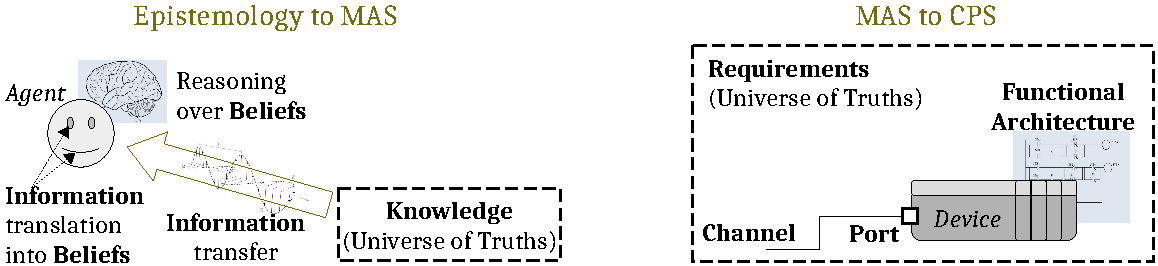
\includegraphics[width=.8\textwidth]{mashyp.pdf}
	\caption{Mapping Epistemological Concepts to (Cyber-Physical) Systems Engineering}
	\label{fig:mashyp}
\end{figure*}

As depicted in Figure~\ref{fig:mashyp}, we relate MAS and CPS as follows.
\begin{itemize}
	\item We consider a System as a hierarchy of agents. So, we map agents
		to \emph{systems, sub-systems, or devices}, depending on the
		granularity of the design. For example, a modeler can model a
		specific device, as in Figure~\ref{fig:mashyp}. In this case,
		the system is not decomposed into sub-systems or devices and
		the device is considered as an agent.
	\item Agents reason over beliefs (i.e. transform beliefs into other
		beliefs) and each \emph{component of a CPS} (system, sub-system,
		or device) is composed by a \emph{functional architecture} that
		transforms input-beliefs into output-beliefs.
	\item Components of a CPS have \emph{ports} to exchange information
		with the outer environment (which may be a sub-system),
		similarly to agents. The transfer of information in a CPS is
		defined by \emph{channels}.
	\item The concept of knowledge is related to the \emph{requirements}
		that, in a factorial way, describe how the CPS shall behave and
		its \emph{physical architecture}.

\end{itemize}

\paragraph{Input and Output Ports}
\begin{figure}[t]
	\centering
	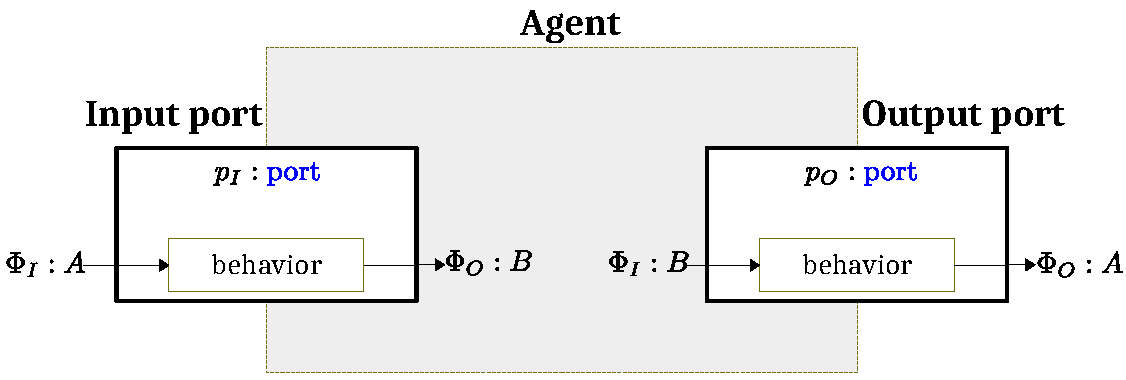
\includegraphics[width=\columnwidth]{IOports.pdf}
	\caption{Input and Output Port of an agent}
	\label{fig:ioports}
\end{figure}
Since the $\abftheory$-framework is a theory of agents, we could consider ports as
agents that allows the exchange of information between a channel and another
agent.  However, we considered a port as a special type of agent to avoid
an \emph{infinite regress}. While a channel transfers information between agents and
a functional architecture elaborate information, a port is simply a connector between
a channel and a functional architecture. One, however, may argue that a similar
connect is needed between a channel and the port itself. While this is not 
excluded by the $\abftheory$-framework, would obviously lead to an infinite
nested structure of ports. In order to avoid this, we assume
that a port doesn't require any other means to transfer information from/to a channel
or from/to a functional architecture. 

\begin{definition}{\bf Input or Output Port --}\label{def:port} 
	A port forwards information from the outside of an agent's boundary to
	the inside (input-port) or vice versa (output-port).  There exist two
	types of ports with the following behavior: an input-port 
	transforms assertions from a sender $s$ ($\rassert{s}{a}$) to beliefs
	of an agent $a$ ($\beliefRegion_a$), while an output-port transforms belief
	into assertion.
\end{definition}
The \emph{quality of a port} is determined by the $\rcc$ relation between the
assertions received or sent and the belief, i.e.
$\Rcc{\rassert{s}{a}}{\beliefRegion_a}$ for the input-port or
$\Rcc{\rassert{r}{*}}{\beliefRegion_a}$ for the output-port.  A port is, in
fact, syntactic sugar to express the relation between assertions and beliefs.
We only define secure input port but the definition of a secure output port is
symmetrical.  Moreover, we note that the definition of an input/output port can
be considered ``secure'', meaning that we implicitly formulated the requirement
that a port always forwards the information without modifying it in any way.
This is assumed because we define a port as if the RCC equality relation holds
between the input/output assertions and the input/output beliefs.  In contrast,
assuming any RCC relation, between inputs and outputs of a port, which is not
an equality can be considered as generating a weaknesses, as we describe in
more details in the next paragraph.

%\begin{definition}{\bf Secure Input Port \fixnote{mv}{chiarirei meglio intuitivamente, magari fuori della definizione, quale sia la differenza tra port e secure port. La differenza è in quell'always?}--}\label{def:secport}
%	A secure input port always allows information as incoming assertions to
%	flow from a sender $s$ to the beliefs (generated by the behavior) of
%	the recipient $a$ (agent).  
%	%If $p_I$ is a secure input port,
%	%$\world\models\varphi$, $\varphi\in\rassert{s}{a}$, and $a$ has the
%	%only input port $p_I$, $\world'\models\beliefRegion_a$ and
%	%$\varphi\in\beliefRegion_a$ for any $\world\modalrelation\world'$.
%\end{definition}

\paragraph{Port Weaknesses}
\begin{theorem}{Port Weaknesses.}
From our definition of ports, it follows that there exist only the following \emph{six}
types of weaknesses, generating six types of insecure port in RCC5 (the
notation is reported for input-ports, i.e. on the left-hand side of the arrow):
\begin{enumerate}[start=1, label={W\arabic*)}]
	\item \emph{replace port}, where assertions reach
		the port but is replaced with different and un-related information
		before passing the boundary 
	\item \emph{drop port}, where assertions reach the
		port but do not pass the boundary of the agent (i.e. do not
		become belief of the agent)
	\item \emph{insertion port}, where some new
		information is believed by $a$ as incoming from the port but
		$s$ didn't send it
	\item \emph{injection port}, where information
		coming from $s$ is substituted with new information which
		becomes believed by $a$
	\item \emph{selective port}, where some information passes the port and
		part is either:
	\begin{enumerate}[start=1, label={W5.\arabic*)}]
		\item drop, 
		\item drop+insert.
	\end{enumerate}
\end{enumerate}
\end{theorem}

\begin{proof}
An input port is, in the $\abftheory$-framework, defined secure as long as the relation
	between the two regions of input assertions $\assertionRegion$ and
	output beliefs $\beliefRegion$ are equal, i.e.
	$\eq{\assertionRegion}{\beliefRegion}$. Therefore, any other relation
	should result in a weakness (related to an insecurity flaw) of that
	input port.  Using RCC5, there exist exactly other $4$ different types
	of relations, one of which is the discrete-from (DR) relation, i.e.
	$\dr{\assertionRegion}{\beliefRegion}$. When two regions are related by
	the DR relations, they have no subregion in common. Let us
	define a function weight $|X|$ such that, for any region $X$, it
	represents the smallest possible cardinality of a (mereo)topological base for
	$X$; where a base is a collection of regions in a (mereo)topology such that
	every open region can be written as union of elements of that base. 
	We distinguish between regions that contain information and regions that
	don't by writing the latter as $\emptyset$.
	\begin{enumerate}
		\item if $\eq{\assertionRegion}{\beliefRegion})$ then either
			$\assertionRegion=\beliefRegion=\emptyset$ (no
			communication) or
			$\assertionRegion=\beliefRegion\neq\emptyset$ (forward
			communication)
		\item if $\dr{\assertionRegion}{\beliefRegion})$ then
			$\assertionRegion=\emptyset\oplus\beliefRegion=\emptyset$
			(we call \emph{insert} the former and \emph{full drop}
			the latter case), or
			$\assertionRegion\neq\emptyset\wedge\beliefRegion\neq\emptyset\wedge\assertionRegion\neq\beliefRegion$
			which we call \emph{replace} (i.e. drop and insert)
		\item if $\pp{\assertionRegion}{\beliefRegion})$ then
			$\beliefRegion$ contains and extend $\assertionRegion$
			which we call \emph{injection}
		\item if $\ppi{\assertionRegion}{\beliefRegion})$ then
			$\assertionRegion$ contains and extend $\beliefRegion$
			which we call \emph{selective drop}
		\item if $\po{\assertionRegion}{\beliefRegion})$ then a part of
			the $\assertionRegion$ is contained in the
			$\beliefRegion$ which is a combination of
			\emph{selective drop and generation}
	\end{enumerate}
\end{proof}

\paragraph{Communication Channels}
\begin{figure}[t]
	\centering
	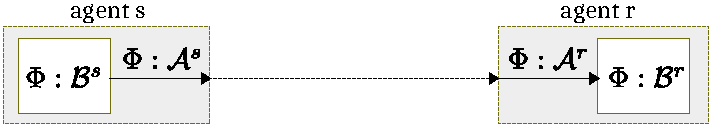
\includegraphics[width=\columnwidth]{channel.pdf}
	\caption{Communication over a Mono-directional Channel}
	\label{fig:channel}
\end{figure}
In this work, we only consider
mono-directional channels and communication but the extension to bi-directional
channel can be considered as the union of two unidirectional channels. A
mono-directional channel is defined by the assertions sent or received (over
the channel). 

We start by considering the difference between a (communication)
mono-directional channel (channel from now on) and an agent, as we did for the
ports, since the $\abftheory$-framework is a theory of agents.  In fact, if a channel
were considered an agent (channel-agent) then the question would be how an
agent would transfer its assertions to the channel-agent. If the channel
between the agent and the channel-agent is again an agent, we would generate an
\emph{infinite regress}. Therefore, we do allow channel-agents but we assume a
finite depth (of detail) for a channel, where there exists a bottom-channel
which is not an agent. For now, we do not constrain a channel-agent in any way
so there is no difference between a channel agent and agent. Therefore,
we consider channels to be bottom-channels,
defined as agents with the pre-defined behavior (i.e. defined in an axiomatic
way) of forwarding any input-assertion as output-assertion, without modifying it\footnote{Nothing
prevents us from introducing additional constraints to the channel as storing
assertions that are transferred over the channel, or filter out some
input-assertions.}. 

\begin{definition}{\bf Mono-directional Channel (bottom-channel) --}\label{def:monochannel}
	A mono-directional channel between two agents ($s \rightarrow r$) is
	defined as an agent whose behavior is (dogmatically) defined as: to
	forward any assertion received from $s$ over an input-port, to  the
	output-port where $r$ is listening to.
\end{definition}
The \emph{quality of a mono-directional} channel is defined as the $\rcc$
relation between the assertions made by the sender and the ones received by the
receiver, i.e. $\Rcc{\assertionRegion_s}{\assertionRegion_r}$.

\paragraph{Channel Weaknesses}
Given that a mono-directional bottom-channel is assumed to be perfectly
forwarding any assertion (as we assumed for ports) from its input-port to its
output-port, there is no insecure behavior but only the combination of the
weaknesses of the input and output port; therefore there exist $(7^2)-2=47$
theoretical configurations ($7^2$ because there are $6$ insecure types of port,
plus $1$ secure type, on both input and output side; and we exclude the
configuration with $2$ secure types as input and output, $-2$); where only 43
are possible. For the sake of readability, we report 6 examples in the
following but the proof by exhaustion over all the possible cases is
straightforward.

\begin{enumerate}[start=6, label={W\arabic*)}]
	\item \emph{secure output port} and \emph{input drop port}
	\item \emph{secure output port} and \emph{input insertion port}
	\item \emph{output drop port} and \emph{input drop port}
	\item \emph{output drop port} and \emph{input insertion port}
	\item \emph{output drop port} and \emph{input secure port}
	\item \emph{output injection port} and \emph{input secure port}
\end{enumerate}

\paragraph{Security Weaknesses -- The RIDI-Hypothesis} 
It is important to note that all the results of the application of the
$\abftheory$-framework to channels (the analysis of the RCC relations
between output and input assertions of an agent)
%$\Rcc{\assertionRegion_o}{\assertionRegion_i}$) 
lead to the same results of the
analysis of a pair of an input and output port.
%(i.e.
%$\Rcc{\beliefRegion_1}{\assertionRegion_2}$ and
%$\Rcc{\assertionRegion_2}{\beliefRegion_3}$)
The same result can be obtained
by analyzing the relation between the outputs of a functional block and the
inputs of another functional block, %($\Rcc{\beliefRegion_o}{\beliefRegion_i}$),
where functional blocks are constituents of the functional architecture as
described afterwards\fixnote{mv}{Questo è difficile da seguire. Non si può spostare a dopo aver definito i functional blocks e il modo in cui li interpretate nel vostro MAS?}.  
As depicted in Figure~\ref{fig:atom}, so far we have
considered information generated by a port $P_I$ and then sent through a
channel $C$ to another (recipient) port $P_O$. In this scenario, where ports and
channels are atomic (otherwise raising infinite regress), we can only
consider the relations between ports and channel; considering both input-port
to channel and channel to output-port.  In fact, the weaknesses of a channel
are defined in terms of the weaknesses of ports.  Io order to define a
functional block without encountering an infinitely recursive definition, we
must reach the same conclusions as for the channel. Therefore, describing the
information as flowing over a channel or in a functional block is purely
syntactic sugar.

We can summarize these results by saying that the relations between assertions
and beliefs, Output assertions of an agent and Input assertions of another
agent, or Output beliefs of a functional block and Input beliefs of another
block can \emph{only} be affected by the following weaknesses: replace, drop,
injection, insertion, selective drop, and selective drop + insertion. 
We call this the RIDI-Hypothesis, being the
four main categories of weaknesses: Replace, Insertion, Drop, Injection. We can,
then, deduce the following security properties to mitigate security weaknesses
of a port or a channel (between ports, functional blocks, or both).
\begin{itemize}
	\item \emph{Order-preserving} -- it shall be known if information is \emph{replaced}
	\item \emph{Availability} -- it shall be known if information is \emph{dropped} or \emph{selectively dropped}
	\item \emph{Integrity} -- it shall be known if information is \emph{injected}
	\item \emph{Authentication} -- it shall be known if information is \emph{inserted}
\end{itemize}
%We can also generalize the weaknesses related to the data flow (i.e. the flow
%of information as assertions or beliefs) as the relation between output-input
%beliefs between functional blocks, output-input assertions of a channel,
%inputs-outputs of a port, as follows.
%\begin{itemize}
%	\item \emph{equal}, expected nominal behavior
%	\item \emph{discrete-from}, drops all the inputs and inserts new malicious data
%	\item \emph{proper part}, selectively drops inputs
%	\item \emph{proper part inverse}, forwards all the inputs but crafts and
%	      inserts new malicious data
%	\item \emph{partial overlap}, selectively drops inputs and inserts new data.
%\end{itemize}


\begin{figure}[t]
	\centering
	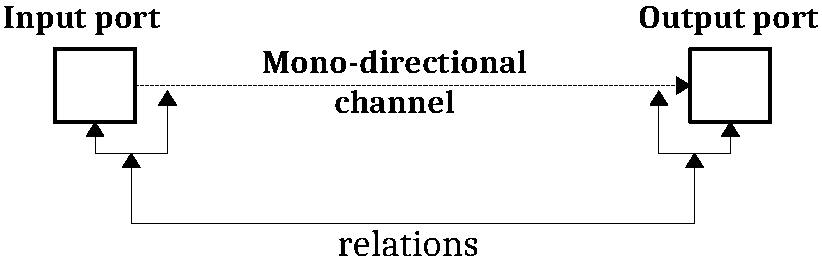
\includegraphics[width=.9\columnwidth]{engineering_relations.pdf}
	\caption{Relations between Ports and Channel}
	\label{fig:atom}
\end{figure}

\paragraph{Functional Architecture}
A functional architecture takes information as input-beliefs and transforms the
information into output-beliefs. Those transformations occurs within the
functional architecture, where functional blocks transforms beliefs into other
beliefs. Similarly to channels, we could consider a functional block as a
functional architecture occurring in an infinite regress. Therefore, we
consider functional blocks as executing an abstract undefined behavior, of
which we only observe the inputs and the resulting outputs (beliefs).

\begin{definition}{\bf Functional Block and Architecture --}\label{def:funblock}
	A functional block of an agent 
	takes a region \fixnote{mv}{Perché qui specificate region mentre nelle definizioni di port e channel non lo facevate?} of input-beliefs and outputs a region of output-beliefs. 
	A functional architecture is an interconnected system of functional blocks.
\end{definition}
It is evident that the quality of a functional block cannot be determined
by the difference between its inputs and outputs (as we did for
ports and channels). The behavior of a functional block
cannot be determined in general; since any functional block will have 
its own purpose based on functional requirements. 
Therefore, while a port semantics is determined by the relation 
between assertions and beliefs, the semantics of a functional block 
is determined by the relation between facts/requirements and I/O beliefs.

In other words, a functional block is a generic agent with no pre-defined general
behavior (while ports and channels have a pre-defined behavior).
In the following, for the sake of simplicity, 
we use the generic region $\beliefRegion$ to refer to the behavior (i.e.
the beliefs generated by the behavior).

\begin{enumerate}[start=50, label={W\arabic*)}]
	\item $\po{\beliefRegion}{\factRegion}$ the component has a Byzantine
		behavior where occasionally outputs the expected output given
		the correct inputs. Not all the inputs are handled properly,
		nor all the expected outputs are always generated when correct
		inputs are given.
	\item $\pp{\beliefRegion}{\factRegion}$ part of the expected outputs are not
	        generated in response to the correct
	        inputs
	\item $\ppi{\beliefRegion}{\factRegion}$ the components
	        correctly performs the expected behavior when the correct
	        inputs are provided but is subject to input
	        injections
	\item $\dr{\beliefRegion}{\factRegion}$ the component
		never performs the expected behavior (e.g. physical
		damage)
\end{enumerate}

\paragraph{Requirements as Facts}
During the specification phase, for any agent, channel, port, functional block
and architecture, there may exist a requirement (fact) predicating over them.
In other words, any requirement is defined as a fact since they must be true in
any design or implementation. As we stated in Section~\ref{sec:theory} and depicted in
Figure~\ref{fig:soundness}, facts are strategic rules that define how
the system shall behave (by specification), while reality may be shown to
be insecure (i.e. diverging from the expected behavior).

\begin{figure}[t]
	\centering
	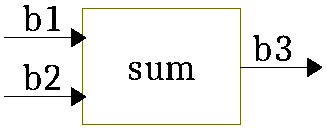
\includegraphics[width=0.3\columnwidth]{sum.pdf}
	\caption{Example of a Functional Block}
	\label{fig:sum}
\end{figure}

As an example, consider a functional block that performs the summation of two
inputs, as in Figure~\ref{fig:sum}, defined by the requirement $r := b_3 = b_1
+ b_2$ for any $b_1$ and $b_2$. The possible relations between the beliefs generated by the behavior of the functional block and
the requirements (i.e. $\Rcc{\beliefRegion}{\factRegion}$ is determined by
the relations between the I/O beliefs $sum(b_1,b_2)=b_3$ and the requirement
$sum(b_1,b_2)=b_1+b_2$, as follows.
\begin{itemize}
	\item $\eq{\beliefRegion}{\factRegion}=\eq{\beliefRegion_3}{\beliefRegion_{1+2}}$, 
		where $\beliefRegion_3$ represents the region of the
		outputs of the functional block $sum$ while the region
		$\beliefRegion_{1+2}$ represents the expected
		outputs of an ideal implementation of the requirement $r$.
		Therefore, the functional block correctly implements the
		requirements.
	\item
		$\dr{\beliefRegion}{\factRegion}=\dr{\beliefRegion_3}{\beliefRegion_{1+2}}$,
		the function block never implements the requirements.
	\item
		$\pp{\beliefRegion}{\factRegion}=\pp{\beliefRegion_3}{\beliefRegion_{1+2}}$, there exist some inputs for which
		the output is incorrect.
	\item $\ppi{\beliefRegion}{\factRegion}=\ppi{\beliefRegion_3}{\beliefRegion_{1+2}}$, there exist some outputs that are not the result of the summation of the inputs but given the correct inputs the function always outputs correctly.
	\item
		$\po{\beliefRegion}{\factRegion}=\po{\beliefRegion_3}{\beliefRegion_{1+2}}$,
		the component has a Byzantine behavior where occasionally
		outputs the expected output given the correct inputs. Not all
		the inputs are handled properly, nor all the expected outputs
		are always generated when correct inputs are given.
\end{itemize}

\paragraph{Assertions and Facts}
The whole reasoning on the relation between beliefs and facts can be duplicated
for the relation between assertions and facts; we cannot appreciate the
difference at this level of abstraction.  If the functional architecture would
be extended to capture the semantics (i.e. the logic) of the communication and
security protocols, with the relation between assertions and facts we would
compare protocol logics with the requirements. We won't consider the verification of
the functional architecture and protocol logic in this paper since we
focus on the architecture specification step of the engineering process
without going into the design of the behavior of agents. We can give an example
but research is needed to apply our theory
to the behavior of agents. 

If we consider a functional block that generates nonces (i.e. number used
only once), the semantics of this block must define a procedure such that 
a freshness requirement holds. By the RIDI-Hypothesis we have that
the following weaknesses may occur:
\begin{itemize}
	\item Replace: the output-nonces of the block are replaced with
		non-fresh numbers
	\item Insert: the output-nonces are concatenated with other numbers,
		resulting in non-fresh nonces. For example, the nonces 110 and
		111 are modified by inserting a 1 and a 0 at the beginning and
		end respectively, resulting in the two identical (and the
		non-fresh) nonces 1110 and 1110
	\item Delete: part of output-nonce is dropped. For example, the last bit of 1101 and 1100 is dropped, resulting in the two equal and non-fresh nonces: 110 and 110.
	\item Inject: substitution at bit level results in non-fresh nonces. For example, 110 becomes 111 becomes equal by flipping either the last 0 of the former nonce or the last 1 of the latter.
\end{itemize}

We summarize our results by categorizing the weaknesses
predicted by our theory into: data-flow-related and functionality-related
weaknesses; as in Table~\ref{tab:weaknesses}.
\begin{table*}[t]
\centering
	\begin{tabular}{c C{.35\textwidth} C{.5\textwidth}} 
		\textbf{RCC5} & \textbf{Quantity: Data Flow} & \textbf{Quality: Requirements Adherence}\\
		\hline 
		EQ & Expected/Nominal & Expected/Nominal\\[.1cm]
	DR & Drops all the inputs and inserts new malicious data & The component never performs/carries the expected behavior/information\\[.1cm]
	PP & Selectively drops inputs & Part of the expected outputs are not generated in response to the correct inputs \\[.1cm]
	PPi& Forwards all the inputs but crafts and inserts new malicious data & The components correctly performs/carries the expected behavior/information when the correct inputs are provided but is subject to input injections \\[.1cm]
	PO & Selectively drops inputs and inserts new data & Byzantine behavior - occasionally outputs the expected output given the correct inputs. Not all the inputs are handled properly, nor all the expected outputs are always generated when correct inputs are given
\end{tabular}
\caption{Weaknesses Categorized~\label{tab:weaknesses}}
\end{table*}

\subsection{Security and Insecurity of a System}
\begin{hypothesis}{\bf System Security Design --}\label{hyp:security}
	A system security design is given by a precise system 
	specification over the physical and functional architectures, that
	uniquely, i.e.  tested against the range of design possible in the
	$\abftheory$-framework, defines the design built on top of those
	requirements.
\end{hypothesis}

\begin{hypothesis}{\bf System Insecurity Design --}\label{hyp:insecurity}
	If, given a system specification as a collection of
	requirements on the system, there exist
	a non-unique design with respect to those requirements, the number of
	equivalent designs that fulfills the requirements quantitatively
	defines the magnitude of insecurity of a system design.
\end{hypothesis}

Based on these hypothesis, we can formulate the concepts of security and
insecurity (in the $\abftheory$-framework) as mathematical equations.  Let us consider a CPS
$S$, represented as a graph $G=\langle V,E\rangle$ where $V$ represents the
set of functional blocks and ports of $S$, and $E\subseteq V\times E$ is the
set of pairs representing the channels and connections (data flows) between
functional blocks. We define $R\subseteq V\times F$, where $F$ is the set
of all the requirements of $S$, and extend $G$ as $G'=\langle E'\times V'\rangle$
with $E'= E\cup R$ and $V'=V\cup F$. Let $\pi: E'\rightarrow RCC$ (where $RCC$ is
the set of relations in the RCC) be
the total function associating an RCC relation to each edge in $G'$, and
$\Pi$ be the set of all different permutations of RCC relations over $E'$
(i.e. $\Pi=\{\langle\pi(e_0)=EQ,\ldots,\pi(e_n)=EQ\rangle,\ldots,\langle \pi(e_0)=DR,\ldots,\pi(e_n)=DR\rangle\}$). If $\sigma:\Pi\rightarrow\{0,1\}$ is an evaluation function
such that $\sigma(p)=1$ (where $p\in\Pi$) iff the input configuration is satisfiable with respect to
the logical theory defining the algebraic structure (mereotopology) and constraints
of the calculus RCC (otherwise $\sigma$ returns $0$), we can define
\begin{displaymath}
	I=\sum_{p\in\{\Pi\setminus\pi_{eq}\}} \sigma(p)
\end{displaymath}
where $\pi_{eq}\in\Pi$ is the output of the function $\pi$ that associates only EQ relations
to any $e\in E'$, and $I\in\mathbb{N}$ represents all the insecurity configurations
of the CPS $S$ where, at least, one of the RCC relations isn't EQ.
In other words, we consider $\pi_{eq}$ as the only secure configuration.

%the insecurity of a system 
%($I$) can be expressed as the following equation.
%\begin{displaymath}
%	I=\prod_{a\in Ag} r_i^{\binom{n}{k}}-\delta_T
%\end{displaymath}
%where $r_i^{\binom{n}{k}}$ represents the number of possible configurations
%(permutations) of an agent (defined as a tuple of RCC relations as in
%Definition~\ref{def:opsystem}) in which at least one of the relation is not EQ.
%$r_i$ represents the RCC relations with arity $k$ between $n$ different regions
%in the $\abftheory$ theory. $\delta_T$ represents the number of configurations
%which are not satisfiable with respect to the logical theory defining the
%algebraic structure (topology) and constraints of the calculus (RCC). $Ag$ is
%the set of all the agents in the system under evaluation and the product
%represents all the unintended, insecure, configurations.  Given that there is
%only $1$ nominal configuration of the system where all the agents are defined
%only with EQ relations (and then the only secure configuration), which can be
%expressed as $sad$ it follows that security can be defined as
%\begin{displaymath}
%	I=\prod_{a\in Ag} r_i^{\binom{n}{k}}-\delta_T
%\end{displaymath}
%
%if $I=0$ the system can be considered secure, 
%otherwise $I$ represents the number of possible insecure configurations, where
%$I\in\mathbb{N}$.

\subsection{Security Risk Assessment}\label{sec:secra}
In order to test our theory we implemented a tool-chain (open-source under the
AGPLv3 license and available at \autocite{v-research2020cybersecurity}) for the
identification of weaknesses and the precise calculation of potential insecure
configurations. The engineering of the $\abftheory$ is summarized in the UML
Class diagram in Figure~\ref{fig:secraclassdiagram} (in appendix). 

\begin{figure}
	\centering
	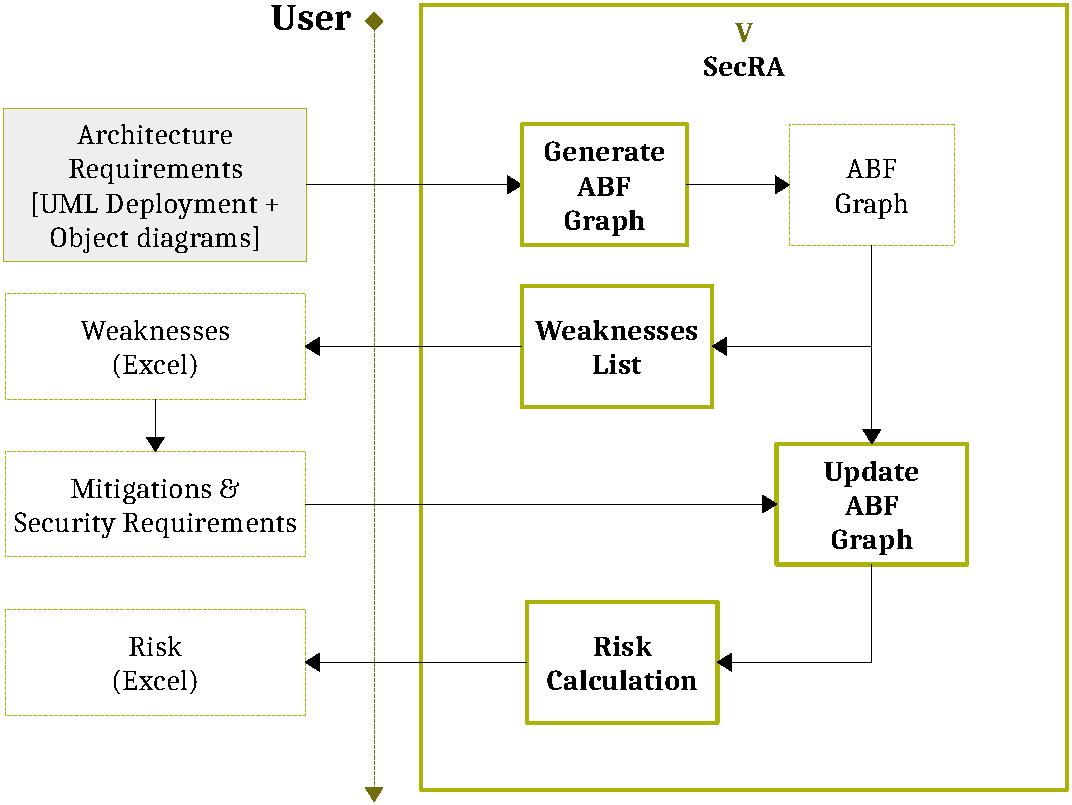
\includegraphics[width=.9\columnwidth]{v-secra.pdf}
	\caption{Security Risk Assessment Tool}
	\label{fig:secra}
\end{figure}
As depicted in Figure~\ref{fig:secra}, the security risk assessment process
starts with the definition of the use cases and architectural requirements; the
specification of a system.  In our process, the specification is manually
translated into a UML design where:
\begin{itemize}
	\item a \emph{Deployment Diagram} describes the \emph{Physical
		Architecture}. Each agent is defined as a Node with (physical)
		ports, and agent's ports are connected via information Flow
		connectors, representing the physical channel.
	\item a \emph{Functional Architecture} is linked to each agent in the
		deployment diagram and is defined by an \emph{Object Diagram}.
		The Object Diagram is composed by Instances of functional
		blocks, connected via information Flow connectors.
	\item the connection between the two diagrams is implemented by
		``sockets'', functional blocks connected to a 
		physical port.
\end{itemize}

The tool generates a graph-like internal structure which represents
the specification (called ABF graph). The ABF graph defines the system as
a number of regions of assertions, beliefs, and facts. Those regions
are connected by a generic relation which is evaluated as follows.
The graph is translated into 
a logical formula that represents the specification in the $\abftheory$-framework and,
along with the axiomatization of the RCC5 calculus, is given as input to the Z3 SMT solver.
The solver identifies all possible configurations of the system and, in turn,
identifies all potential weaknesses. 
The internal structures of the tool
can be viewed as PDF and the results are reported into an Excel file.
The Excel file also reports the total number of configurations as indicating
the security risk associated to the specification. A user can change the status
of each weakness in the Excel file, from the initial (default) status (open)
to ``mitigated''. As a consequence, the risk is re-calculated on-the-fly, i.e.
without the need of running the tool again, based on annotations and formulas 
in the Excel file.

In our approach, security requirements are not imposed by the
specification but are automatically extracted by our tool as potential weaknesses.
Those weaknesses are related to the different insecure configurations 
of the specified system. 

The risk matrix is often defined as a function of 
likelihood and impact of attacks. We suggest
that security weaknesses are all equally likely to be exploited
if there's a connection between the weakness and the asset that
an attacker wants to impact. 

\paragraph{Case Studies}
We report the results of the evaluation of a water level reader (sensor ad-hoc example). 
\begin{figure}
	\centering
	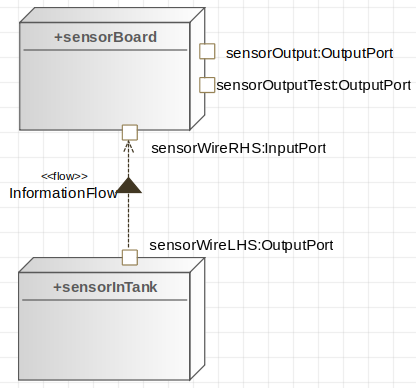
\includegraphics[width=.6\columnwidth]{eng_cs1.png}
	\caption{Water Level Reader Deployment Diagram}
	\label{fig:eng_cs1}
\end{figure}
As in Figure~\ref{fig:eng_cs1}, we defined 2 agents: sensorInTank and sensorBoard,
which represent the physical reader that needs to be placed in a tank of water, and 
the board that interprets the readings and outputs them as digital signals.
The two components are connected by a wire.
\begin{figure}
	\centering
	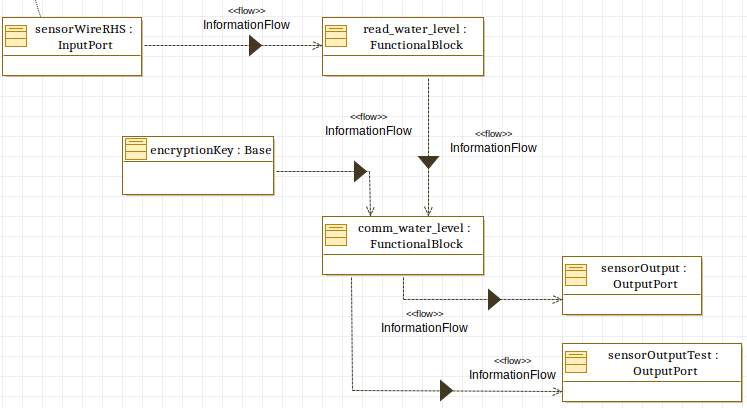
\includegraphics[width=.9\columnwidth]{internal_cs1.png}
	\caption{Sensor Board Object Diagram}
	\label{fig:int_cs1}
\end{figure}
In Figure~\ref{fig:int_cs1} we report the functional architecture that
receives the incoming communications from the sensor in the tank, and 
communicates them encrypted.
\begin{figure*}
	\centering
	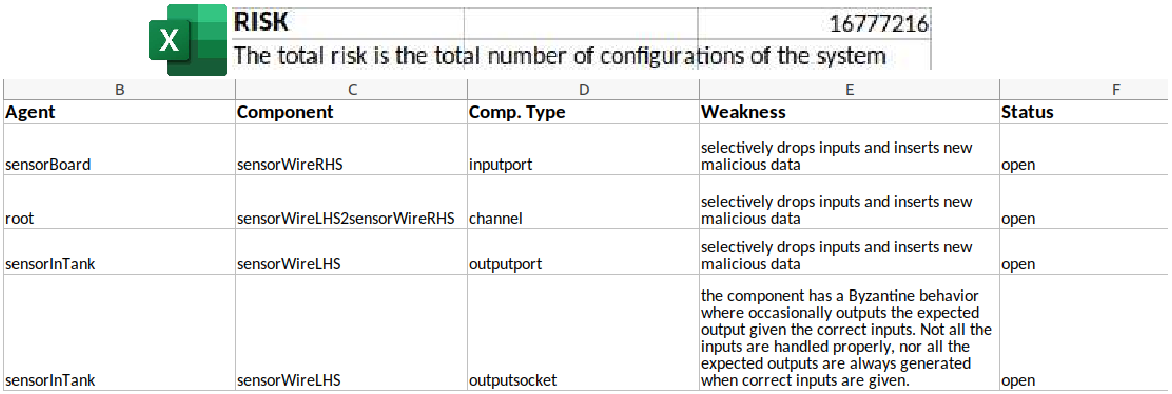
\includegraphics[width=.7\textwidth]{results_excel.pdf}
	\caption{Partial View of the results in the Excel file}
	\label{fig:results}
\end{figure*}
The results, summarized in Figure~\ref{fig:results} reports more than 16 millions
possible scenarios in which at least one component diverge from the specification.

%\section{Discussions}\label{sec:discussion}
%\paragraph{Abstraction Level}
%The level of abstraction is always a concern when it comes to the definition of
%a system model.  In this paper, we justified our assumptions on the atomicity
%of ports, channels, and functional blocks but nothing prevents a modeler to
%consider other atomic element of the system specification and design.  Those
%additional elements may detail the system and may change the syntactic sugar we
%defined; however, it won't change the underlying (semantic) reasoning unless
%another calculus is used (instead of RCC).  Furthermore, other Infosec
%properties may be considered, such as authenticity or non-repudiation. We,
%however, leave them as future development.
%
%\paragraph{$\abftheory$ Falsification} The theory we developed can be falsified
%by providing an experiment that shows a weaknesses not predicted by the
%$\abftheory$-framework, or by showing that the weaknesses predicted for a certain
%experiment are impossible to realize.  This theory, however, needs to be
%detailed to be applicable to a full engineering process (we only cover the
%first steps).  We propose the following complete process as a draft for
%potential next steps in this direction.
%\begin{enumerate}
%\item System Specification
%\item Architecture Design
%\item Security Risk Assessment and Security Requirement Extraction
%\item Design Refinement, where the semantics of the functional behavior and
%	communication protocols are defined 
%\item Security Requirement Extension, based on the design refinement
%\item Verification of Security Requirements (data flow, behaviors, \& protocol
%	logic)
%\item Software Prototype Implementation/Synthesis
%\item Automated Security Testing (abstract test-suite generation \&
%	concretization)
%\item Hardware Prototype Implementation
%\item Automated Security Testing
%\item Penetration Testing
%  \end{enumerate}
%
%\paragraph{Relation with DY}
%The DY attacker model has been extensively
%used for the identification of logical weaknesses in security protocols.
%Our theory should predict all possible weaknesses which, in turn,
%should enable all the attacks identified by the DY model. 
%A proof that the two theories/models correctly predicts
%(or lacks in predicting) weaknesses and related protocol flaws would
%connect risk assessment and protocol verification, the first
%two steps of the secure engineering of systems.

\section{Conclusion and Future Works}
\fixnote{mv}{Se ho capito bene, detto a parole mie, quello che il vostro
approccio permette di fare, dati requisiti e architettura del sistema, è di
elencare in maniera sistematica tutti i "punti" in cui potrebbero sorgere dei
problemi. Spiegherei un po' meglio, qui nelle conclusioni o nella sezione
precedente, come questo approccio dovrebbe essere usato nella pratica... Voglio
dire che non mi sembra necessariamente in opposizione ad altri approcci ma
magari può integrarsi a questi.  Inoltre quando parlate dei passi successivi,
ad esempio il considerare la generazione di test cases, se avete già qualche
idea su come procedere, potreste discuterne brevemente.}
We proposed a foundational theory on security, arguing that
security-related issues are not related to the maliciousness of an agent but to
the vagueness of the security controls on the engineering processes.
The current state-of-the-art processes allow, given a specification,
an engineer to design the system in such a way that security issues arise due to the lack
of proper security risk assessment processes.
Those design, again, lack of security verification processes based on a solid 
security foundational theory and then permit the generation of insecure implementation.
The security verification and test-case generation will be the focus of our next steps.

We conclude that the problem of security is a problem related to the 
many possible design and, in turn, implementation given a specification.
The problem is related to the epistemological search for truth,
where the challenge is to relate information and belief to human knowledge.
Scientifically, generalizing the human to an agent, the problem is
to relate assertions and beliefs, to facts. From an engineering standpoint,
by generalizing the concept of agents as architectural subsystems, the
problem is to link channels (and ports) and functional architectures to 
requirements.

\section*{Acknowledgment}
We thank Katia Santac\`a for the help in the development of the initial ideas, and for
the helpful discussions that allowed us to make this step forward.

\appendix
The Class Diagram for the Engineering of the $\abftheory$-framework is reported in
Figure~\ref{fig:secraclassdiagram}. A \emph{specification} of a CPS is viewed
as an aggregation of \emph{architectures} which can describe the functional or
physical requirements. The physical components of the architecture are
input/output \emph{ports} and \emph{channels} (aggregations of pairs of ports)
while \emph{functional blocks} are the only constituents of the functional
architecture. All of the classes are abstract except input/output ports and
functional blocks. Therefore, agents (which represents sub-systems or
components) are composed by ports and functional blocks, as an aggregation of 
architectures.

\begin{sidewaysfigure*}
	\centering
	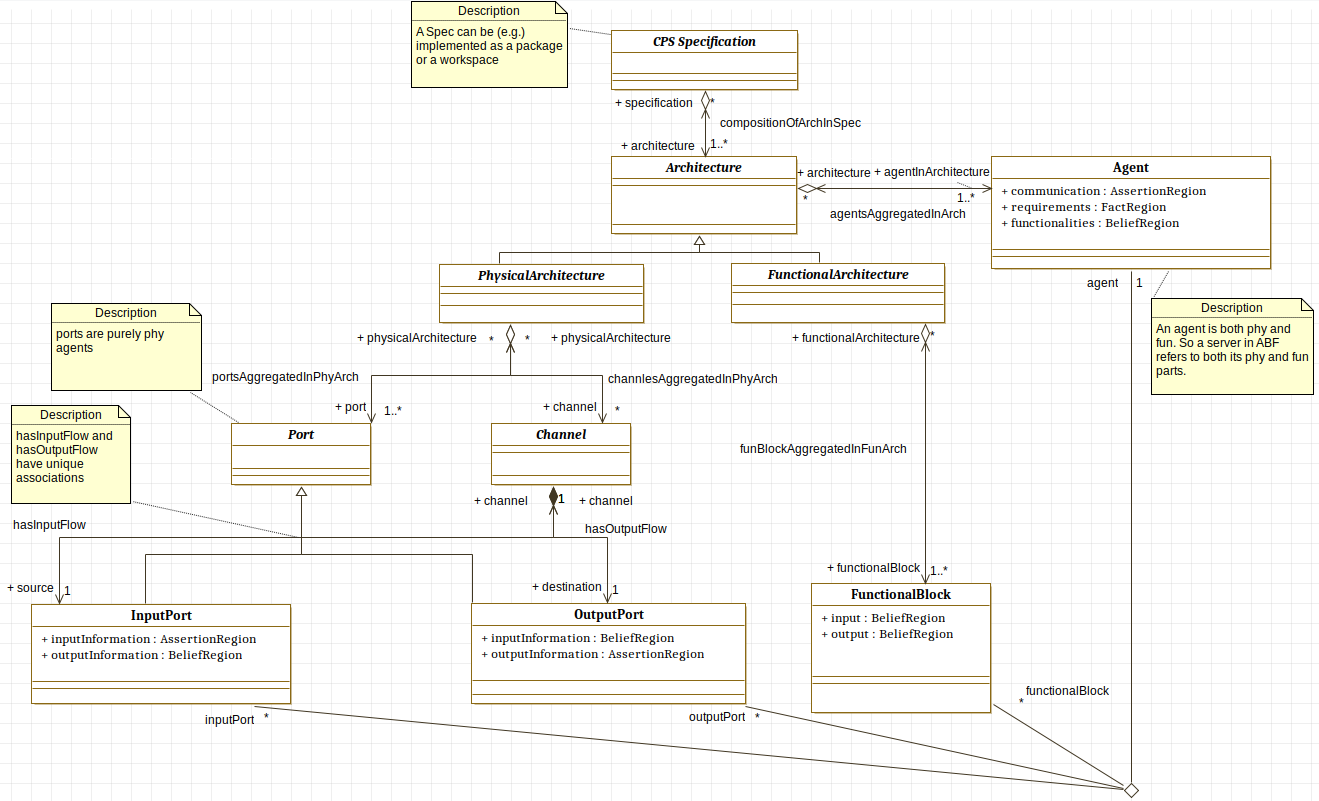
\includegraphics[width=\textwidth]{secra_classDiagram.png}
	\caption{Security Risk Assessment -- Class Diagram}
	\label{fig:secraclassdiagram}
\end{sidewaysfigure*}
\printbibliography

% trigger a \newpage just before the given reference
% number - used to balance the columns on the last page
% adjust value as needed - may need to be readjusted if
% the document is modified later
%\IEEEtriggeratref{8}
% The "triggered" command can be changed if desired:
%\IEEEtriggercmd{\enlargethispage{-5in}}

%\bibliographystyle{IEEEtran}
%\bibliography{../literature}

\end{document}
